% This is samplepaper.tex, a sample chapter demonstrating the
% LLNCS macro package for Springer Computer Science proceedings;
% Version 2.21 of 2022/01/12
%
\documentclass[runningheads]{llncs}
%
\usepackage[T1]{fontenc}
% T1 fonts will be used to generate the final print and online PDFs,
% so please use T1 fonts in your manuscript whenever possible.
% Other font encondings may result in incorrect characters.
%
\usepackage{hyperref}
\usepackage{graphicx}
\usepackage{proof}
\usepackage{tikz-cd}
% \tikzcdset{scale cd/.style={every label/.append style={scale=#1},
%     cells={nodes={scale=#1}}}}
\tikzcdset{row sep/normal=0.22cm}
\tikzcdset{column sep/normal=0.02cm}
% Used for displaying a sample figure. If possible, figure files should
% be included in EPS format.
%
% If you use the hyperref package, please uncomment the following two lines
% to display URLs in blue roman font according to Springer's eBook style:
\usepackage{color}
\renewcommand\UrlFont{\color{blue}\rmfamily}
\urlstyle{rm}
%
\usepackage{amsmath,amssymb,amsfonts}%

\newlength{\alphabetheight}
\settoheight{\alphabetheight}{Ap}

\newlength{\alphabetdepth}
\settodepth{\alphabetdepth}{Ap}

\newcommand{\agdahen}{%
  \begingroup
  \raisebox{-\alphabetdepth}
  {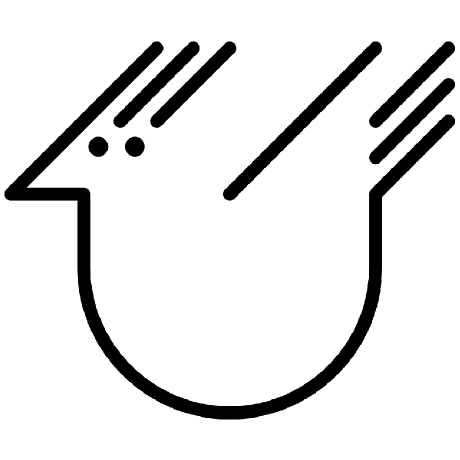
\includegraphics[height=1em]{agdahen.png}}%
  \endgroup
}

\newcommand{\agdaurl}{https://github.com/cswphilo/nonassociative-Lambek}
%\newcommand{\agdahref}{a7dbb4bc7ca9251d8d08d24d5ab5922cdb6ce1c1}
\newcommand{\agdahref}{116dbb88fbe4bcaf942368a01e045a80c7b1951f}
\newcommand{\agdaref}[1]{\href{\agdaurl/blob/\agdahref/code/#1}{\agdahen}}

%% macros for typesetting
\newcommand{\udl}[1]{\underline{#1}}
\newcommand{\proofbox}[1]{\begin{array}{c} #1 \end{array}}

%% macros for math symbols
\newcommand{\ot}{\otimes}
\newcommand{\cdast}{\circledast}
\newcommand{\Larr}{\Leftarrow}
\newcommand{\Rarr}{\Rightarrow}
\newcommand{\btleft}{\blacktriangleleft}
\newcommand{\btright}{\blacktriangleright}
\newcommand{\sls}{\slash}
\newcommand{\bsls}{\backslash}
\newcommand{\mc}[1]{\mathcal{#1}}
\newcommand{\mf}[1]{\mathsf{#1}}
\newcommand{\vars}[1]{\mf{var} (#1)}
\newcommand{\gs}[1]{\sigma_{X} (#1)}
\newcommand{\GG}{\Gamma}
\newcommand{\Gg}{\gamma}
\newcommand{\GD}{\Delta}
\newcommand{\Gd}{\delta}
\newcommand{\Gl}{\lambda}

%% macros for acronyms 
\newcommand{\MIP}{\textsf{MIP}}
\newcommand{\MIPeq}{{\textsf{MIP}{\circeq}}}
\newcommand{\FL}{$\mathtt{FL}$}
\newcommand{\Lam}{$\mathtt{L}$}
\newcommand{\NL}{$\mathtt{NL}$}

%% macros for derivations
\newcommand{\vd}{\vdash}
\newcommand{\ax}{\mathsf{ax}}
\newcommand{\tl}{{\otimes}\mathsf{L}}
\newcommand{\tr}{{\otimes}\mathsf{R}}
\newcommand{\Ll}{{\Larr}\mathsf{L}}
\newcommand{\Lr}{{\Larr}\mathsf{R}}
\newcommand{\Rl}{{\Rarr}\mathsf{L}}
\newcommand{\Rr}{{\Rarr}\mathsf{R}}
\newcommand{\cut}{\mf{cut}}

%% commands for Agda stuff
\newcommand{\At}{\mathsf{At}}
\newcommand{\at}{\mathsf{at}}
\newcommand{\Fma}{\mathsf{Fma}}
\newcommand{\data}{\mathsf{data}}
\newcommand{\Tree}{\mathsf{Tree}}
\newcommand{\Path}{\mathsf{Path}}
\newcommand{\pathT}[1]{\mathsf{Path} ~ #1}
\newcommand{\append}{+\!\!+}
\newcommand{\Sub}{\mathsf{sub}}
\newcommand{\sub}[2]{\mathsf{sub} ~ #1 ~ #2}
\newcommand{\where}{\mathsf{where}}
\newcommand{\Set}{\mathsf{Set}}
\newcommand{\record}{\mathsf{record}}
\newcommand{\field}{\mathsf{field}}
\newcommand{\subst}{\mathsf{subst}}
\newcommand{\Same}{\mathsf{Same}}
\newcommand{\ContainsLeft}{{\in}\mathsf{Left}}
\newcommand{\ContainsRight}{{\in}\mathsf{Right}}
\newcommand{\LeftRight}{\mathsf{Disj}}
\newcommand{\subcases}{\mathsf{SubEq}}
\newcommand{\oneeqtwo}{\mathsf{case}_1}%{\mathsf{1{\equiv}2}}
\newcommand{\twogtLone}{\mathsf{case}_2}%{\mathsf{2{>}L1}}
\newcommand{\twogtRone}{\mathsf{case}_3}%{\mathsf{2{>}R1}}
\newcommand{\onegtLtwo}{\mathsf{case}_4}%{\mathsf{1{>}L2}}
\newcommand{\onegtRtwo}{\mathsf{case}_5}%{\mathsf{1{>}R2}}
\newcommand{\oneLtwoR}{\mathsf{case}_6}%{\mathsf{1\sls \bsls 2}}
\newcommand{\oneRtwoL}{\mathsf{case}_7}%{\mathsf{2\sls \bsls 1}}
\newcommand{\subeq}{\mathsf{subeq}}
\newcommand{\inT}{\in^{\mf{T}}}


\newcommand{\niccolo}[1]{\textcolor{red}{NV: #1}}
\newcommand{\cheng}[1]{\textcolor{blue}{CSW: #1}}

\begin{document}
%
\title{An Agda Formalization of Nonassociative Lambek Calculus and Its Metatheory}
%
\titlerunning{Agda Formalization of Nonassociative Lambek Calculus}
% If the paper title is too long for the running head, you can set
% an abbreviated paper title here
%
\author{Niccol{\`o} Veltri\orcidID{0000-0002-7230-3436} \and
Cheng-Syuan Wan \orcidID{0000-0003-2053-1688}}
%
\authorrunning{N. Veltri and C.-S. Wan}
% First names are abbreviated in the running head.
% If there are more than two authors, 'et al.' is used.
%
\institute{Tallinn University of Technology, Tallinn, Estonia
\\
\email{\{niccolo,cswan\}@cs.ioc.ee}}
%
\maketitle              % typeset the header of the contribution
%
\begin{abstract}
  This paper presents a formalization of the nonassociative Lambek calculus in the Agda proof assistant. %, focusing on two major proof-theoretic properties: cut admissibility and Maehara interpolation. 
  The sequent calculus for this logic has sequents with binary trees as antecedents, in which formulae are stored as leaves. The shape of the antecedents creates subtleties when proving logical properties, since in many cases one needs to analyze equalities involving sequentially-composed trees. We formally characterize these equalities and show how to employ the resulting technical lemma to prove cut admissibility and the Maehara interpolation properly, which implies Craig interpolation. We show that both the cut rule and the interpolation procedure are well-defined wrt.\ a certain notion of equivalence of derivations. We additionally prove a proof-relevant version of Maehara interpolation, exhibiting the interpolation procedure as a right inverse of the admissible cut rule. 
  %Our work, especially the case distinction type defined here, aims to serve as a foundation for further research and formalization on nonassociative Lambek calculus.
\keywords{nonassociative Lambek calculus \and Agda \and cut admissibility \and Maehara interpolation \and proof-relevant interpolation}
\end{abstract}
%
%
%

\section{Introduction}
From the perspective of sequent calculus, substructural logics are characterized by the absence of at least one structural rule. A notable instance is Lambek's syntactic calculus \cite{lambek:mathematics:58}, which forbids the structural rules of weakening, contraction and exchange. Its non-associative variant, also introduced by Lambek \cite{Lambek1961}, further disallows associativity.
% also introduced by Lambek \cite{Lambek1961}, disallows associativity as well.
The Lambek calculus (both its associative and nonassociative variants) has been extensively studied in the literature, especially for its linguistic applications \cite{moot:categorial:2012}.
%While Lambek calculus has different presentations, including axiomatic (or syntactic), natural deduction, and sequent calculus, we focus primarily on the proof-theoretic aspect, specifically the sequent calculus formulation.

In its sequent calculus presentation, sequents in the associative Lambek calculus (\Lam) are of the form $\GG \vd C$, where $\GG$ is a \emph{list} of formulae and $C$ is a single formula, while sequents in the nonassociative Lambek calculus (\NL) are of the form $T \vd C$ where $T$ is a \emph{binary tree} in which formulae are stored in the leaves.
This structural difference makes the proofs of logical properties for \NL\ trickier than for the associative variant.
For example, when proving cut admissibility, in certain cases, one must determine whether the cut formula coincides with the principal formula of the conclusion. For \Lam, the flat antecedents make the situation clear: there are three possibilities--either the cut formula is to the left of the principal formula, to the right, or it is the principal formula itself.

For \NL, the situation is more involved, as there are more cases to examine. %while the case distinction follows similar principles, the hierarchical tree structure obscures these relationships.
For example, consider the proof of cut admissibility, in which we wish to compose the derivations of sequents $U \vdash D$ and $\mc{C}[D] \vd C$. Here $\mc{C}$ is a context, i.e. a tree with a hole, and $\mc{C}[D]$ is the tree resulting from plugging the formula $D$ in the hole. If the derivation of the second sequent ends with an application of the left $\Rl$-introduction rule,
then its antecedent is of the form $\mc{C}'[U' , A \Rarr B]$ for some context $\mc{C}'$, tree $U'$ and formulae $A,B$ (where $\mc{C}'[U',A\Rarr B]$ is the tree arising from substituting the tree $(U', A\Rarr B)$ in context $\mc{C}'$). This means that we are given an equality of trees $\mc{C}[D]=\mc{C}'[U',A \Rarr B]$ and we need to precisely characterize the structural relationship between the cut formula $D$ and the tree $(U,A \Rarr B)$ within the contexts $\mc{C}$ and $\mc{C}'$.
%$\ot$-introduction rule, then its antecedent is of the form $T'[A \ot B]$ for some context $T'$ and formulae $A,B$. This means that we are given an equality of trees $T[D]=T'[A \ot B]$ and we need to precisely characterize the structural relationship between the tensor formula $A \ot B$ and the cut formula $D$ within these trees.
This relationship is not as simple as in the associative Lambek calculus, it involves a more complex splitting of the contexts from which more cases arise.

We can intuitively understand what occurs in the proof of cut admissibility, since it is not too difficult to compute all possible cases. However, what about more complex properties?  For example, consider proving that the admissible cut rule is associative, i.e. the two ways of cutting three sequents of the form $U \vdash D$, $\mc{C}[D] \vdash E$ and $\mc{C}'[E] \vdash C$ produce equal derivations. Because of the large number of cases arising from the induction on the shape of derivations and, mostly, from the analysis of equalities of trees discussed in the previous paragraph, establishing the associativity of cut becomes very challenging to perform with pen and paper, as it is hard to keep track of all the possible cases to consider.
On the other hand, interactive theorem provers are very good tools for dealing with large inductive proofs and keeping track of all existing proof obligations.

%This need leads us to consider a formal verification of the \NL. Our approach involves paths in trees, allowing each subtree to be represented as a substitution along a path in the original tree. This transforms the problem of determining relative positions between different subtrees into a formalizable question about the relationship between two paths in a tree.
%For example, if two formulae $A$ and $B$ are in a tree with paths $p_1$ and $p_2$ respectively, and these paths are disjoint (diverging at some point), then there must exist some common path $q$ and two paths $q_1$ and $q_2$ after divergence such that $p_1$ equals the path concatenation of $q$ and $q_1$, while $p_2$ equals the concatenation of $q$ and $q_2$.

In this work, we present the formalization of the sequent calculus for \NL\ and its metatheory in the Agda proof assistant. We start by formally describing all possible cases arising from equalities of sequentially-composed trees of the form $\mc{C}[U]=\mc{C}'[U']$, which is the main technical lemma that we employ in the proof of logical properties. In particular, cut admissibility and properties of the admissible cut rule: associativity, commutativity and unitality wrt.\ the axiom rule.
%Formalization of mathematics and logics has become a trend in both theoretical computer science and mathematics. While there are many suitable proof assistants (e.g., Agda, Coq, HOL4, and Lean), we choose Agda because its code is more mathematical in style and the process of proving theorems resembles providing algorithms to compute desired terms in the target type.
%\cheng{Maybe here can be some more explanation about why formalization is important}.

%Within proof theory, interpolation properties serve as fundamental property of a logic and of interests by different logicians.
We then present the formal proof of the Maehara interpolation property, originating from Maehara's proof of Craig interpolation \cite{craig:interpolation:1957} for classical logic \cite{maehara1961}.
Maehara's method has been applied and adapted to several logics, especially to substructural logics that admit a cut-free sequent calculus \cite{ono:proof:nonclassical:1998}. The Maheara interpolation property states that, given a sequent $\mc{C}[U] \vdash C$, there exist a formula $D$ and derivations of sequents $U \vdash D$ and $\mc{C}[D] \vdash C$, such that all the atomic formulae appearing in $D$ appear also in $U$, as well as in $\mc{C},C$.
More precisely, we formalize a proof-relevant (in the sense of \v{C}ubri{\'c} \cite{vcubric1993results,Cubric1994} and Saurin \cite{Saurin2024}) variant of Maehara interpolation: we aim to capture not only the existence of interpolants but also their relationship to the admissible cut rule. In order to achieve this, we first introduce an equivalence relation $\circeq$ on derivations, capturing all the possible permutative conversions. We then show that both the cut rule and the interpolation procedure are well-defined wrt. to the relation $\circeq$. %e.g. if we interpolate on two equivalent derivations, then their interpolants are identical and the corresponding derivations are pairly equivalent.
 Then we show that the interpolation procedure is a right inverse of the admissible cut rule, in the sense that running the interpolation algorithm on a derivation $f$ of a sequent $\mc{C}[U] \vdash C$ and successively cutting the resulting two derivations along the interpolant formula results in a derivation that is $\circeq$-related to $f$.
%i.e. if we interpolate on two equivalent derivations, then their interpolants are identical and the corresponding derivations are pairly equivalent.

%In this paper, we formalize \NL\ and prove properties in Agda: $(i)$ cut-elimination, $(ii)$ Maehara interpolation, $(iii)$ proof-relevant interpolation, and $(iv)$ \linebreak well-definedness of the Maehara interpolation procedure with respect to equivalence of derivations.
Summarizing, this work makes the following contributions: $(i)$ we formalize a technical lemma for dealing with equalities of the form $\mc{C}[U] = \mc{C}'[U']$; $(ii)$ we employ the lemma to formally define effective procedures for cut admissibility and Maehara (and consequently Craig) interpolation; $(iii)$ we prove proof-relevant versions of the latter, by introducing an equivalence of derivations $\circeq$ and formally establishing many properties of the defined procedures: cut is associative, commutative and unital; cut and interpolation are well-defined wrt. $\circeq$; interpolation is a right inverse of cut. We notice that contribution $(iii)$ is completely novel in the study of the metatheory of \NL, not only its mechanization in a proof assistant.
%The paper proceeds as follows. We begin with the foundations of our formalization, including definitions of trees, paths in trees, substitutions, and case distinctions for identifying relationships between paths. Next, we introduce the sequent calculus of \NL\ and formalize cut-elimination. The subsequent section addresses equivalence of derivations and properties of the $\cut$ rule.
%In the final sections, we formally prove Maehara interpolation and proof-relevant interpolation to demonstrate that our formalization provides a correct and usable strategy. It is worth noting that the proof-relevant interpolation results presented here are novel contributions to the study of \NL.

\paragraph{Related work.}
% \\
% Several previous works have formalized aspects of nonassociative Lambek calculus:
There is some previous work on the formalization of \NL\ in proof assistants. Chapter 4 of Anoun et al.'s tutorial \cite{anoun2004proof} presents a Coq formalization of the nonassociative Lambek calculus, covering axiomatic calculus, natural deduction and sequent calculus. Tian \cite{tian2017formalized} ported the above Coq formalization to HOL4. Kokke \cite{kokke2017formalising} formalized the nonassociative Lambek-Grishin calculus in Agda. %However, their work focused on axiomatic calculus, where both the antecedent and succedent are single formulae, in contrast to the sequent calculus with tree as antecedents that we formalize.
These earlier formalizations primarily focus on implementing the calculi and proving cut admissibility with potential linguistic applications in mind.
%Our project takes a more proof-theoretic perspective, formally verify  focusing on the equational theory of proofs. We formalize not only cut-elimination but also extend to Maehara interpolation, proof-relevant interpolation, and demonstrate that Maehara interpolation is well-defined with respect to equivalence of derivations.

The Craig interpolation property for intuitionistic logic has been formalized in Isabelle/HOL by Ridge \cite{ridge:2006} and in Nominal Isabelle by Chapman et al. \cite{ChapmanMU08}. For  classical logic, there is a formalization in Isabelle/HOL by Michealis and Nipkow \cite{michealis:2017}. Recently,  F{\'{e}}r{\'{e}}e and van Gool \cite{feree:2023} have formalized uniform interpolation for intuitionistic logic in Coq, which was extended to a class of modal logics by F{\'{e}}r{\'{e}}e et al. \cite{feree:24}. As far as we know, there are no formalized proofs of Craig/Maehara interpolation for substructural logics in the literature.

We would like to add that the (pen-and-paper, non-formalized) proof of Maehara interpolation for \NL\ is uncommon in the literature, as we were unable to find a reference for it. For \NL\ (and its extensions with modalities, additive connectives, etc.) researchers have traditionally been interested in other interpolation properties, involving a different condition on atomic formulae, which are useful for establishing the finite model property and the relationship between Lambek grammars and context-free grammars \cite{buszkowski1986generative,kandulski1988equivalence,jager:04,buszkowski:2009,buszkowski:2010,lin:14}.
%Our method is more akin to traditional Maehara's method because our interest lies in a more refined analysis based on equivalence of derivations.

\paragraph{Formalization}
All our constructions have been formalized in Agda.
The code is freely available online at \url{https://github.com/cswphilo/nonassociative-Lambek/tree/main/code}.
Throughout the paper each result is accompanied by a clickable link, in the form of the Agda logo (\agdahen), directing to the corresponding line in the Agda code.


\section{Basics on Trees}\label{sec:agda:base}
In this section, we introduce the core elements of our Agda formalization: trees, paths within trees and substitutions.
We mainly aim at proving a technical lemma characterizing equalities of the form $\mc{C}[U] = \mc{C}'[U']$. Intuitively, this lemma states that either $(i)$ $U = U'$, $(ii)$ $U$ is a subtree of $U'$, $(iii)$ $U'$ is a subtree of $U$, or  $(iv)$ $U$ and $U'$ are disjoint subtrees. Formally, one needs also to characterize the shape of contexts $\mc{C}$ and $\mc{C}'$ in all these cases.
%We focus particularly on the key formalization of determining the relative positions of subtrees of a tree.
%It is designed to precisely characterize whether two subtrees with different representations are identical, one contains the other, or they diverge after some common path.
The technical lemma is fundamental to our subsequent formalization of cut admissibility and Maehara interpolation for \NL, as well as for establishing properties of these procedures.

\subsection{Formulae, Trees, Substitutions}
Formulae of \NL\ are inductively generated by the grammar
$$A, B ::= X \ | \ A \Larr B \ | \ B \Rarr A \ | \ A \ot B$$
where $X$ is drawn from a set $\mathsf{At}$ of atomic formulae,
$\ot$ is multiplicative conjunction and $\Larr$,$\Rarr$ are left and right implications (also called residuals).
In our formalization, we postulate the existence of a type $\At$ of atomic formulae. We consistently use letters $X, Y, Z$ to denote atomic formulae.
The type $\Fma$ (\agdaref{Fma.agda\#L17}) of formulae is defined as the following inductive type:
\[
\begin{array}{rl}
  \multicolumn{2}{l}{\data \:\:  \Fma : \Set \:\: \where} \\
  \;\; \at &: \At \to \Fma \\
  \;\; \_{\Larr}\_ &: \Fma \to \Fma \to \Fma \\ 
  \;\; \_{\Rarr}\_ &: \Fma \to \Fma \to \Fma \\ 
  \;\; \_{\ot}\_ &: \Fma \to \Fma \to \Fma \\
\end{array}
\]
Underscores indicate infix operators, e.g. $A \ot B$ is a formula for any $A,B : \Fma$.

In the literature on \NL\ \cite{moot:categorial:2012}, trees (also called structures) are defined inductively by the grammar $T,U ::= A \mid (T, U)$ where $A$ is a single formula.
Contexts are trees with a hole, inductively specified by the grammar   $\mathcal{C} ::= [\bullet] \mid (\mathcal{C}, T) \mid (T, \mathcal{C})$. 
In our formalization, we conflate the two notions and define a type $\Tree$ (\agdaref{Fma.agda\#L25}) of trees possibly containing more than one hole. This representation becomes convenient in the specification of the technical lemma.
We will see in Section \ref{sec:calculus} that allowing the presence of holes in trees is unproblematic, as antecedents of valid sequents are necessarily free of holes.
%We formalize the type $\Tree$ of trees as the following inductive type:
\[
\begin{array}{rl}
  \multicolumn{2}{l}{\data \:\:  \Tree : \Set \:\: \where} \\
  \;\; \bullet &: \Tree \\
  \;\; \eta &: \Fma \to \Tree \\
  \;\; \_{\cdast}\_ &: \Tree \to \Tree \to \Tree \\
\end{array}
\]
The base constructor $\bullet$ corresponds to a hole, the constructor $\eta$ corresponds to a leaf containing a formula, while $\cdast$ is the node constructor.
%\niccolo{Maybe we can change $\eta$ to $\mathsf{fma}$ and $\cdast$ to a special comma/semicolon, to keep notation closer to the usual one.}

%Our definition more closely resembles the definition of contexts in \cite{moot:categorial:2012}. This approach facilitates smoother proofs and allows us to define derivations using the same type. This definition does not introduce inconsistent derivations since the axiom sequents are defined with non-empty antecedents (see Section \ref{sec:calculus} for the formal sequent calculus).

We introduce a type $\pathT{T}$ (\agdaref{Fma.agda\#L38}) whose terms are paths in the tree $T$. These are sequences of left ($\btleft$) or right ($\btright$) moves from the root node of $T$ to a hole $\bullet$.
The type family $\Path$ is the following inductive type family:
\[
\begin{array}{rl}
  \multicolumn{2}{l}{\data \:\:  \Path : \Tree \to \Set \:\: \where} \\
  \;\; \bullet &: \pathT{\bullet} \\
  \;\; \_{\btleft}\_ &: \forall ~ \{T\} ~ (p : \pathT{T}) ~ U \to \pathT{(T \cdast U)} \\
  \;\; \_{\btright}\_ &: \forall ~ T ~ \{U\} ~ (p : \pathT{U}) \to \pathT{(T \cdast U)}
\end{array}
\]
Curly brackets are used in Agda to denote implicit arguments.
The constructor name $\bullet$ is overloaded: we have that $\bullet : \Tree$ is a tree consisting of a single hole and $\bullet : \pathT{\bullet}$ is the unique path to the hole in that tree.

In the literature on \NL\ \cite{moot:categorial:2012}, the substitution $\mc{C}[U]$ of a tree $U$ into a hole of a context $\mc{C}$ is defined by structural recursion on $\mc{C}$:
\begin{displaymath}
  \begin{array}{rcl}
  [\bullet][U] &=& U
  \\
  (\mc{C},V)[U] &=& (\mc{C}[U],V)
  \\
  (V,\mc{C})[U] &=& (V , \mc{C}[U])
  \end{array}
\end{displaymath}
%We use $T[\bullet]$ to denote a context and $T[U]$ to abbreviate $subst(T[\bullet], U)$.
In Agda, the substitution function replaces a hole in $T$, specified by a given path, by another tree $U$. This is defined by pattern-matching on the path (\agdaref{Fma.agda\#L45}).
%If $T$ has $n+1$ holes, the resulting tree $\sub{p}{U}$ has $n$ holes.
\[
\begin{array}{ll}
  \multicolumn{2}{l}{\Sub : \forall \{T\} \to \pathT{T} \to \Tree \to \Tree}
  \\[2pt]
  \sub{\bullet}{U} &= U
  \\
  \sub{(p \btleft V)}{U} &= \sub{p}{U} \cdast V
  \\
  \sub{(V \btright p)}{U} &= V \cdast \sub{p}{U} 
\end{array}
\]

%For any tree $U$, the substitution operation that replaces $\bullet$ with $U$ follows the path specified above.
Two paths $p : \pathT{T}$ and $q : \pathT{U}$ can be concatenated, resulting in a path $p \append ~ q : \pathT{(\sub{p}{U})}$ in the tree obtained by substituting $U$ in the hole specified by path $p$. Concatenation is defined by pattern-matching on $p$ (\agdaref{Fma.agda\#L52}).

\begin{example}\label{example:tree:and:path}
Consider the tree $T = (\eta X ~ \cdast ~ \bullet) \cdast ~ \eta Y$, which contains a single hole.
The path to the hole is $p = (\eta X \btright \bullet) \btleft \eta Y$, which indicates that, starting from the root node, we take one step to the left followed by one step to the right, after which we reach the hole.
%\[
%  % https://q.uiver.app/#q=WzAsNSxbMCw0LCJcXGV0YSBYIl0sWzEsMiwiXFxjZGFzdCJdLFsyLDQsIlxcY2RvdCJdLFsyLDAsIlxcY2Rhc3QiXSxbMywyLCJcXGV0YSBZIl0sWzEsMCwiIiwwLHsic3R5bGUiOnsiaGVhZCI6eyJuYW1lIjoibm9uZSJ9fX1dLFsxLDIsIiIsMix7InN0eWxlIjp7ImhlYWQiOnsibmFtZSI6Im5vbmUifX19XSxbMywxLCIiLDIseyJzdHlsZSI6eyJoZWFkIjp7Im5hbWUiOiJub25lIn19fV0sWzMsNCwiIiwwLHsic3R5bGUiOnsiaGVhZCI6eyJuYW1lIjoibm9uZSJ9fX1dXQ==
%\begin{tikzcd}
%% [sep=tiny]
%	&& \cdast \\
%	\\
%	& \cdast && {\eta Y} \\
%	\\
%	{\eta X} && \bullet
%	\arrow[no head, from=1-3, to=3-2]
%	\arrow[no head, from=1-3, to=3-4]
%	\arrow[no head, from=3-2, to=5-1]
%	\arrow[no head, from=3-2, to=5-3]
%\end{tikzcd}
%\]
%  Recall the tree and path in Example \ref{example:tree:and:path}. We call them $T$ and $p$, respectively.
  Given another tree $U = \eta Z \cdast \bullet$ and a path $q = \eta Z \btright \bullet$ in $U$, the concatenation of paths $p$ and $q$ is $p \append ~ q = (\eta X \btright (\eta Z \btright \bullet)) \btleft \eta Y$, which is a path in the tree $\sub{p}{U} = (\eta X ~ \cdast ~ (\eta Z \cdast \bullet)) \cdast ~ \eta Y$.
\end{example}

Given paths $p : \pathT{T}$ and $q : \pathT{U}$, substituting a tree $V$ in the concatenation $p \append~ q$ is the same as first substituting $V$ in $q$ and then substituting the result in $p$, i.e. $\sub{(p \append ~q)}{V} \equiv \sub{p}{(\sub{q}{V})}$ (\agdaref{Fma.agda\#L61}),
where $\equiv$ is Agda's propositional equality type.
Agda allows the extension of its evaluation relation with new computation rules using the flag \texttt{{-}{-}rewriting}.
This enabled us to turn the latter propositional equality into a judgemental one.
This is only used to \emph{simplify} the proofs of cut admissibility and Maehara interpolation (and their properties).
All our formalized results remain valid when the equality is propositional instead of judgemental.

Path concatenation is also associative, i.e. $(p \append~ q) \append~ r \equiv p \append~ (q \append~ r)$ for $p : \pathT{T}$, $q : \pathT{U}$ and $r : \pathT{V}$ (\agdaref{Fma.agda\#L69}). Notice that the latter is a well-formed equality type, since the term $(p \append~ q) \append~ r$ has type $\pathT{(\sub{(p \append ~q)}{V})}$ while $p \append~ (q \append~ r)$ has type $\pathT{(\sub{p}{(\sub{q}{V})})}$, but these types are judgementally equal (due to the discussion in the previous paragraph).

\subsection{Equality of Substituted Trees}
When proving cut admissibility and Maehara interpolation for \NL, a common step is determining all possible cases arising from equalities of the form $\mc{C}_1[U_1] = \mc{C}_2[U_2]$. In our Agda formalization, these will be propositional equalities of the form $\sub{p_1}{U_1} \equiv \sub{p_2}{U_2}$, where $p_1$ and $p_2$ are paths in some trees $T_1$ and $T_2$ respectively.
%different presentations of the same tree. For cut-elimination, this involves finding the relationship between the principal formula of the endsequent and the cut formula. For interpolation, it concerns the relationship with the interpolating tree. 
%\begin{example}\label{example:same:tree:diff:sub}
%  Consider the tree $T$ in Example \ref{example:tree:and:path}, we can represent it in at least two equivalent ways: $\sub{((\eta X \cdast \bullet) \btright \bullet)}{\eta Y}$ or $\sub{(\bullet \btleft \eta Y)}{(\eta X \cdast \bullet)}$.
%\end{example}
%We formalize this common process by constructing record types that encompass all possible scenarios where the same tree can be presented in two different ways.
This subsection is dedicated to providing a concrete characterization of the equality type $\sub{p_1}{U_1} \equiv \sub{p_2}{U_2}$, i.e. we are after a type $\subcases ~ p_1 ~ p_2 ~ U_1 ~ U_2$ that is equivalent to $\sub{p_1}{U_1} \equiv \sub{p_2}{U_2}$. We only need to employ one direction of this equivalence (\agdaref{Fma.agda\#L143}):
\begin{equation}\label{eq:subeq}
\begin{array}{l}
 \subeq : \forall ~ \{T_1 ~ T_2 \} ~ U_1 ~ U_2 ~ (p_1 : \pathT{T_1}) ~ (p_2 : \pathT{T_2})
  \\
  \quad \to (eq : \sub{p_1}{U_1} \equiv \sub{p_2}{U_2}) \to \subcases ~ p_1 ~ p_2 ~ U_1 ~ U_2
\end{array}
\end{equation}

The type $\subcases ~ p_1 ~ p_2 ~ U_1 ~ U_2$ (\agdaref{Fma.agda\#L133}) is the disjoint union of all the  cases that can occur, of which there are 7:
\[
\begin{array}{rll}
  \multicolumn{3}{l}{\data \:\:  \mathsf{SubEq} \:\: (p_1 : \pathT{T_1})~ (p_2 : \pathT{T_2})~ (U_1 ~ U_2 : \Tree) : \Set \:\: \where} \\
  \;\; \oneeqtwo &: \Same ~ p_1 ~ p_2 ~ U_1 ~ U_2 &\to \subcases ~ p_2 ~ p_1~ U_1 ~ U_2 \\
  \;\; \twogtLone &: \ContainsLeft ~ p_1 ~ p_2 ~ U_1 ~ U_2 &\to \subcases ~ p_2 ~ p_1~ U_1 ~ U_2 \\
  \;\; \twogtRone &: \ContainsRight ~ p_1 ~ p_2 ~ U_1 ~ U_2 &\to \subcases ~ p_2 ~ p_1~ U_1 ~ U_2 \\
  \;\; \onegtLtwo &: \ContainsLeft ~ p_2 ~ p_1 ~ U_2 ~ U_1 &\to \subcases ~ p_2 ~ p_1~ U_1 ~ U_2 \\
  \;\; \onegtRtwo &: \ContainsRight ~ p_2 ~ p_1 ~ U_2 ~ U_1 &\to \subcases ~ p_2 ~ p_1~ U_1 ~ U_2 \\
  \;\; \oneLtwoR &: \LeftRight ~ p_1 ~ p_2 ~ U_1 ~ U_2 &\to \subcases ~ p_2 ~ p_1~ U_1 ~ U_2 \\
  \;\; \oneRtwoL &: \LeftRight ~ p_2 ~ p_1 ~ U_2 ~ U_1 &\to \subcases ~ p_2 ~ p_1~ U_1 ~ U_2
\end{array}
\]
Let us go through them one by one.
%To this aim, we fix two paths $p_1 : \pathT{T_1}$ and $p_2 : \pathT{T_2}$ and two trees $U_1$ and $U_2$, such that $\sub{p_1}{U_1}$ is propositionally equal to $\sub{p_2}{T_2}$. There are four possibilities:
%\\
\begin{case}[$U_1$ is equal to $U_2$]
In this case, $T_1$ must be equal to $T_2$ and $p_1$ equal to $p_2$.
We collect this information in the record type $\Same ~ p_1 ~ p_2 ~ U_1 ~ U_2$ (\agdaref{Fma.agda\#L85}).
\[
\begin{array}{rl}
  \multicolumn{2}{l}{\record \:\:  \Same ~(p_1 : \pathT{T_1})~ (p_2 : \pathT{T_2})~ (U_1 ~ U_2 : \Tree) : \Set \:\: \where} \\
%  \multicolumn{2}{l}{\quad \mathsf{constructor} ~ \mathsf{same}} \\
  \multicolumn{2}{l}{\quad \field} \\
  \;\; \quad eqT &: T_1 \equiv T_2 \\
  \;\; \quad eqU &: U_1 \equiv U_2 \\
  \;\; \quad eqp &: \subst ~ \Path ~ eqT ~ p_1 \equiv p_2
\end{array}
\]
Terms of this type are triples consisting of three equalities about the outer trees, the inner trees used for substitution into holes, and paths, respectively.
Notice that paths $p_1$ and $p_2$ have different types, so to be able to equate them one needs to first substitute $T_2$ for the equal tree $T_1$ in the type of $p_1$. This is what the application of $\subst$ in the type of $eqp$ is used for.
\end{case}
\begin{case}[$U_1$ contains $U_2$ in its left subtree]
In this case, there exist trees $W_1$ and $W_2$ and a path $q$ in $W_1$ such that $U_1$ is equal to the tree $\sub{q}{U_2} \cdast W_2$.
Moreover, $p_2$ is equal to the concatenation of $p_1$ with $q \btleft W_2$.
Visually, an example of a tree $\sub{p_2}{U_2}$ (equal to $\sub{p_1}{U_1})$ for this case is
\[
\begin{tikzcd}[row sep=0.16cm]
	&&& \cdast \\
	\\
	&& \cdast && {V_1} \\
	\\
	& \cdast && {W_2} \\
	\\
	{V_2} && {U_2}
	\arrow[no head, from=1-4, to=3-3]
%	\arrow["{p_1}"', shift right, color={rgb,255:red,214;green,92;blue,92}, no head, from=1-4, to=3-3]
	\arrow[no head, from=1-4, to=3-5]
	\arrow[no head, from=3-3, to=5-2]
%	\arrow[shift right, draw={rgb,255:red,214;green,92;blue,92}, no head, from=3-3, to=5-2]
	\arrow[no head, from=3-3, to=5-4]
	\arrow[no head, from=5-2, to=7-1]
%	\arrow["q", shift left, color={rgb,255:red,214;green,92;blue,92}, no head, from=5-2, to=7-3]
	\arrow[no head, from=5-2, to=7-3]
\end{tikzcd}
\]
We can break apart this tree and identify all the relevant component trees and paths (the latter marked in red):
\begin{equation*}\label{eq:containsleft}
\begin{array}{c}
  T_1 = 
\begin{tikzcd}[row sep=0.16cm]
	&&& \cdast \\
	\\
	&& \bullet && {V_1} \\
	\arrow[no head, from=1-4, to=3-3]
	\arrow["{p_1}"', shift right, color={rgb,255:red,214;green,92;blue,92}, no head, from=1-4, to=3-3]
	\arrow[no head, from=1-4, to=3-5]
\end{tikzcd}
\qquad
T_2 =
\begin{tikzcd}[row sep=0.16cm]
	&&& \cdast \\
	\\
	&& \cdast && {V_1} \\
	\\
	& \cdast && {W_2} \\
	\\
	{V_2} && {\bullet}
	\arrow[no head, from=1-4, to=3-3]
	\arrow["{p_1}"', shift right, color={rgb,255:red,214;green,92;blue,92}, no head, from=1-4, to=3-3]
	\arrow[no head, from=1-4, to=3-5]
	\arrow[no head, from=3-3, to=5-2]
	\arrow[shift right, draw={rgb,255:red,214;green,92;blue,92}, no head, from=3-3, to=5-2]
	\arrow[no head, from=3-3, to=5-4]
	\arrow[no head, from=5-2, to=7-1]
	\arrow["q", shift left, color={rgb,255:red,214;green,92;blue,92}, no head, from=5-2, to=7-3]
	\arrow[no head, from=5-2, to=7-3]
\end{tikzcd}
\\
W_1 = 
\begin{tikzcd}[row sep=0.16cm]
	&&& \cdast \\
	\\
	&& {V_2} && {\bullet} \\
	\arrow[no head, from=1-4, to=3-3]
	\arrow["{q}", shift left, color={rgb,255:red,214;green,92;blue,92}, no head, from=1-4, to=3-5]
	\arrow[no head, from=1-4, to=3-5]
\end{tikzcd}
\qquad
U_1 =
\begin{tikzcd}[row sep=0.16cm]
	&& \cdast \\
	\\
	& \cdast && {W_2} \\
	\\
	{U_2} && {V_2}
	\arrow[no head, from=1-3, to=3-2]
%        \arrow[shift right, color={rgb,255:red,214;green,92;blue,92}, no head, from=1-3, to=3-2]
	\arrow[no head, from=1-3, to=3-4]
%	\arrow["{q}"', shift right, color={rgb,255:red,214;green,92;blue,92}, no head, from=3-2, to=5-1]
	\arrow[no head, from=3-2, to=5-1]
	\arrow[no head, from=3-2, to=5-3]        
\end{tikzcd}
\end{array}
\end{equation*}
%in the left subtree of $U_1$ without $U_2$ (for brevity, when we say ``left subtree of $U_1$'', we mean the left subtree of $U_1$ minus $U_2$).
%Let $W_1$ and $W_2$ be the left and right subtrees of $U_1$, respectively.
%Let us visualize this situation on an example.
%Consider the tree $T_1 = \bullet \cdast V_1$, for some tree $V_1$, with $p_1 = \bullet \btleft V_1$.
%Consider trees $T_1$ and $\sub{p_1}{U_1}$ with the following structure (here $V_1$ is an arbitrary tree):
%\[
%\arraycolsep=1.5cm
%\begin{array}{cc}
%  % https://q.uiver.app/#q=WzAsMyxbMSwwLCJcXGNkYXN0Il0sWzAsMiwiXFxidWxsZXQiXSxbMiwyLCJWXzEiXSxbMCwxLCIiLDAseyJzdHlsZSI6eyJoZWFkIjp7Im5hbWUiOiJub25lIn19fV0sWzAsMSwicF8xIiwyLHsib2Zmc2V0IjoxLCJjb2xvdXIiOlswLDYwLDYwXSwic3R5bGUiOnsiaGVhZCI6eyJuYW1lIjoibm9uZSJ9fX0sWzAsNjAsNjAsMV1dLFswLDIsIiIsMix7InN0eWxlIjp7ImhlYWQiOnsibmFtZSI6Im5vbmUifX19XV0=
%\begin{tikzcd}
%	& \cdast \\
%	\\
%	\bullet && {V_1}
%	\arrow[no head, from=1-2, to=3-1]
%	\arrow["{p_1}"', shift right, color={rgb,255:red,214;green,92;blue,92}, no head, from=1-2, to=3-1]
%	\arrow[no head, from=1-2, to=3-3]
%\end{tikzcd}
%&
%% https://q.uiver.app/#q=WzAsNSxbMiwwLCJcXGNkYXN0Il0sWzEsMiwiXFxjZGFzdCJdLFszLDIsIlZfMSJdLFswLDQsIldfMSJdLFsyLDQsIldfMiJdLFswLDEsIiIsMCx7InN0eWxlIjp7ImhlYWQiOnsibmFtZSI6Im5vbmUifX19XSxbMCwxLCJwXzEiLDIseyJvZmZzZXQiOjEsImNvbG91ciI6WzAsNjAsNjBdLCJzdHlsZSI6eyJoZWFkIjp7Im5hbWUiOiJub25lIn19fSxbMCw2MCw2MCwxXV0sWzAsMiwiIiwyLHsic3R5bGUiOnsiaGVhZCI6eyJuYW1lIjoibm9uZSJ9fX1dLFsxLDMsIiIsMix7InN0eWxlIjp7ImhlYWQiOnsibmFtZSI6Im5vbmUifX19XSxbMSw0LCIiLDIseyJzdHlsZSI6eyJoZWFkIjp7Im5hbWUiOiJub25lIn19fV1d
%\begin{tikzcd}
%	&& \cdast \\
%	\\
%	& \cdast && {V_1} \\
%	\\
%	{W_1} && {W_2}
%	\arrow[no head, from=1-3, to=3-2]
%	\arrow["{p_1}"', shift right, color={rgb,255:red,214;green,92;blue,92}, no head, from=1-3, to=3-2]
%	\arrow[no head, from=1-3, to=3-4]
%	\arrow[no head, from=3-2, to=5-1]
%	\arrow[no head, from=3-2, to=5-3]
%\end{tikzcd}
%\\
%(T_1)
%&
%(\sub{p_1}{U_1})
%\end{array}
%\]
%Since $U_1$ contains $U_2$ as a subtree, we can diagram $\sub{p_2}{T_2}$ as shown in the left diagram below, where the blue path represents $p_2$. The right diagram illustrates how $p_2$ extends $p_1$. We denote the path in $W_1$ as $q$
%\begin{equation}\label{eq:ContainsLeft:p1p2}
%  \arraycolsep=1cm
%\begin{array}{cc}
%% https://q.uiver.app/#q=WzAsNyxbMCw2LCJVXzIiXSxbMSw0LCJcXGNkYXN0Il0sWzIsNiwiVl8yIl0sWzIsMiwiXFxjZGFzdCJdLFszLDQsIldfMiJdLFszLDAsIlxcY2Rhc3QiXSxbNCwyLCJWXzEiXSxbMSwwLCIiLDAseyJzdHlsZSI6eyJoZWFkIjp7Im5hbWUiOiJub25lIn19fV0sWzEsMiwiIiwyLHsic3R5bGUiOnsiaGVhZCI6eyJuYW1lIjoibm9uZSJ9fX1dLFszLDEsIiIsMix7InN0eWxlIjp7ImhlYWQiOnsibmFtZSI6Im5vbmUifX19XSxbMyw0LCIiLDAseyJzdHlsZSI6eyJoZWFkIjp7Im5hbWUiOiJub25lIn19fV0sWzUsMywiIiwwLHsic3R5bGUiOnsiaGVhZCI6eyJuYW1lIjoibm9uZSJ9fX1dLFs1LDYsIiIsMix7InN0eWxlIjp7ImhlYWQiOnsibmFtZSI6Im5vbmUifX19XSxbNSwzLCIiLDAseyJvZmZzZXQiOjEsImNvbG91ciI6WzI0MCw2MCw2MF0sInN0eWxlIjp7ImhlYWQiOnsibmFtZSI6Im5vbmUifX19XSxbMywxLCIiLDAseyJvZmZzZXQiOjEsImNvbG91ciI6WzI0MCw2MCw2MF0sInN0eWxlIjp7ImhlYWQiOnsibmFtZSI6Im5vbmUifX19XSxbMSwwLCIiLDAseyJvZmZzZXQiOjEsImNvbG91ciI6WzI0MCw2MCw2MF0sInN0eWxlIjp7ImhlYWQiOnsibmFtZSI6Im5vbmUifX19XV0=
%\begin{tikzcd}[row sep=0.16cm]
%	&&& \cdast \\
%	\\
%	&& \cdast && {V_1} \\
%	\\
%	& \cdast && {W_2} \\
%	\\
%	{U_2} && {V_2}
%	\arrow[no head, from=1-4, to=3-3]
%	\arrow[shift right, draw={rgb,255:red,92;green,92;blue,214}, no head, from=1-4, to=3-3]
%	\arrow[no head, from=1-4, to=3-5]
%	\arrow[no head, from=3-3, to=5-2]
%	\arrow[shift right, draw={rgb,255:red,92;green,92;blue,214}, no head, from=3-3, to=5-2]
%	\arrow[no head, from=3-3, to=5-4]
%	\arrow[no head, from=5-2, to=7-1]
%	\arrow[shift right, draw={rgb,255:red,92;green,92;blue,214}, no head, from=5-2, to=7-1]
%	\arrow[no head, from=5-2, to=7-3]
%\end{tikzcd}
%&
%% https://q.uiver.app/#q=WzAsNyxbMCw2LCJVXzIiXSxbMSw0LCJcXGNkYXN0Il0sWzIsNiwiVl8yIl0sWzIsMiwiXFxjZGFzdCJdLFszLDQsIldfMiJdLFszLDAsIlxcY2Rhc3QiXSxbNCwyLCJWXzEiXSxbMSwwLCIiLDAseyJzdHlsZSI6eyJoZWFkIjp7Im5hbWUiOiJub25lIn19fV0sWzEsMiwiIiwyLHsic3R5bGUiOnsiaGVhZCI6eyJuYW1lIjoibm9uZSJ9fX1dLFszLDEsIiIsMix7InN0eWxlIjp7ImhlYWQiOnsibmFtZSI6Im5vbmUifX19XSxbMyw0LCIiLDAseyJzdHlsZSI6eyJoZWFkIjp7Im5hbWUiOiJub25lIn19fV0sWzUsMywiIiwwLHsic3R5bGUiOnsiaGVhZCI6eyJuYW1lIjoibm9uZSJ9fX1dLFs1LDYsIiIsMix7InN0eWxlIjp7ImhlYWQiOnsibmFtZSI6Im5vbmUifX19XSxbMywxLCIiLDAseyJvZmZzZXQiOjEsImNvbG91ciI6WzI0MCw2MCw2MF0sInN0eWxlIjp7ImhlYWQiOnsibmFtZSI6Im5vbmUifX19XSxbNSwzLCJwXzEiLDIseyJvZmZzZXQiOjEsImNvbG91ciI6WzAsNjAsNjBdLCJzdHlsZSI6eyJoZWFkIjp7Im5hbWUiOiJub25lIn19fSxbMCw2MCw2MCwxXV0sWzEsMCwicSIsMix7Im9mZnNldCI6MSwiY29sb3VyIjpbMCw2MCw2MF0sInN0eWxlIjp7ImhlYWQiOnsibmFtZSI6Im5vbmUifX19LFswLDYwLDYwLDFdXV0=
%\begin{tikzcd}[row sep=0.16cm]
%	&&& \cdast \\
%	\\
%	&& \cdast && {V_1} \\
%	\\
%	& \cdast && {W_2} \\
%	\\
%	{U_2} && {V_2}
%	\arrow[no head, from=1-4, to=3-3]
%	\arrow["{p_1}"', shift right, color={rgb,255:red,214;green,92;blue,92}, no head, from=1-4, to=3-3]
%	\arrow[no head, from=1-4, to=3-5]
%	\arrow[no head, from=3-3, to=5-2]
%	\arrow[shift right, draw={rgb,255:red,92;green,92;blue,214}, no head, from=3-3, to=5-2]
%	\arrow[no head, from=3-3, to=5-4]
%	\arrow[no head, from=5-2, to=7-1]
%	\arrow["q"', shift right, color={rgb,255:red,214;green,92;blue,92}, no head, from=5-2, to=7-1]
%	\arrow[no head, from=5-2, to=7-3]
%\end{tikzcd}
%\end{array}
%\end{equation}
%The trees $T_2$ and $U_1$ are the following:
%\begin{equation}\label{eq:ContainsLeft:T2U1}
%\arraycolsep=1cm
%\begin{array}{cc}
%% https://q.uiver.app/#q=WzAsNyxbMCw2LCJcXGJ1bGxldCJdLFsxLDQsIlxcY2Rhc3QiXSxbMiw2LCJWXzIiXSxbMiwyLCJcXGNkYXN0Il0sWzMsNCwiV18yIl0sWzMsMCwiXFxjZGFzdCJdLFs0LDIsIlZfMSJdLFsxLDAsIiIsMCx7InN0eWxlIjp7ImhlYWQiOnsibmFtZSI6Im5vbmUifX19XSxbMSwyLCIiLDIseyJzdHlsZSI6eyJoZWFkIjp7Im5hbWUiOiJub25lIn19fV0sWzMsMSwiIiwyLHsic3R5bGUiOnsiaGVhZCI6eyJuYW1lIjoibm9uZSJ9fX1dLFszLDQsIiIsMCx7InN0eWxlIjp7ImhlYWQiOnsibmFtZSI6Im5vbmUifX19XSxbNSwzLCIiLDAseyJzdHlsZSI6eyJoZWFkIjp7Im5hbWUiOiJub25lIn19fV0sWzUsNiwiIiwyLHsic3R5bGUiOnsiaGVhZCI6eyJuYW1lIjoibm9uZSJ9fX1dXQ==
%\begin{tikzcd}[row sep=0.16cm]
%	&&& \cdast \\
%	\\
%	&& \cdast && {V_1} \\
%	\\
%	& \cdast && {W_2} \\
%	\\
%	\bullet && {V_2}
%	\arrow[no head, from=1-4, to=3-3]
%	\arrow[no head, from=1-4, to=3-5]
%	\arrow[no head, from=3-3, to=5-2]
%	\arrow[no head, from=3-3, to=5-4]
%	\arrow[no head, from=5-2, to=7-1]
%	\arrow[no head, from=5-2, to=7-3]
%\end{tikzcd}
%&
%% https://q.uiver.app/#q=WzAsNSxbMCw0LCJVXzIiXSxbMSwyLCJcXGNkYXN0Il0sWzIsNCwiVl8yIl0sWzIsMCwiXFxjZGFzdCJdLFszLDIsIldfMiJdLFsxLDAsIiIsMCx7InN0eWxlIjp7ImhlYWQiOnsibmFtZSI6Im5vbmUifX19XSxbMSwyLCIiLDIseyJzdHlsZSI6eyJoZWFkIjp7Im5hbWUiOiJub25lIn19fV0sWzMsMSwiIiwyLHsic3R5bGUiOnsiaGVhZCI6eyJuYW1lIjoibm9uZSJ9fX1dLFszLDQsIiIsMCx7InN0eWxlIjp7ImhlYWQiOnsibmFtZSI6Im5vbmUifX19XV0=
%\begin{tikzcd}[row sep=0.16cm]
%	&& \cdast \\
%	\\
%	& \cdast && {W_2} \\
%	\\
%	{U_2} && {V_2}
%	\arrow[no head, from=1-3, to=3-2]
%	\arrow[no head, from=1-3, to=3-4]
%	\arrow[no head, from=3-2, to=5-1]
%	\arrow[no head, from=3-2, to=5-3]
%\end{tikzcd}
%\\
%(T_2)
%&
%(U_1)
%\end{array}  
%\end{equation}
This information is collected in the record type $\ContainsLeft~p_1 ~ p_2 ~ U_1 ~ U_2$ (\agdaref{Fma.agda\#L101}):
\[
\begin{array}{ll}
  \multicolumn{2}{l}{\record \:\:  \ContainsLeft ~(p_1 : \pathT{T_1})~ (p_2 : \pathT{T_2})~ (U_1 ~ U_2 : \Tree) : \Set \:\: \where} \\
%  \multicolumn{2}{l}{\quad \mathsf{constructor} ~ \mathsf{gt}} \\
  \multicolumn{2}{l}{\quad \field} \\
  \;\; \quad \{W_1 ~ W_2 \} &: \Tree \\
  \;\; \quad q   &: \pathT{W_1} \\
  \;\; \quad eqT &: T_2 \equiv \sub{p_1}{(W_1 \cdast W_2)} \\
  \;\; \quad eqU &: U_1 \equiv \sub{(q \btleft W_2)}{U_2} \\
  \;\; \quad eqp &: \subst ~ \Path ~ eqT ~ p_2 \equiv p_1 \append ~ (q \btleft W_2)
\end{array}
\]
Terms of this type are tuples consisting of trees $W_1$ and $W_2$ (which are implicit), as well as a path $q : \pathT{W_1}$, which indicates how to extend $p_1$.
Additionally, there are three equalities characterizing $T_2$, $U_1$, and $p_2$.%, as depicted in (\ref{eq:containsleft}).
%The first and second equalities correspond to our observations from the left and right diagrams in (\ref{eq:ContainsLeft:T2U1}), respectively.
%The third equality reflects what we observed in the right diagram of (\ref{eq:ContainsLeft:p1p2}).
\end{case}
\begin{case}[$U_1$ contains $U_2$ in its right subtree]
This case is similar to the previous one, with the difference that now $q$ is a path in $W_2$ and $U_1$ is equal to $W_1 \cdast \sub{q}{U_2}$.
Moreover, $p_2$ is equal to the concatenation of $p_1$ with $W_1 \btright q$.
This information is collected in the record type $\ContainsRight~p_1 ~ p_2 ~ U_1 ~ U_2$ (\agdaref{Fma.agda\#L110}):
\[
\begin{array}{ll}
  \multicolumn{2}{l}{\record \:\:  \ContainsRight~(p_1 : \pathT{T_1})~ (p_2 : \pathT{T_2}) ~ (U_1 ~ U_2 : \Tree) : \Set \:\: \where} \\
  \multicolumn{2}{l}{\quad \field} \\
  \;\; \quad \{W_1 ~ W_2 \} &: \Tree \\
  \;\; \quad q   &: \pathT{W_2} \\
  \;\; \quad eqT &: T_2 \equiv \sub{p_1}{(W_1 \cdast W_2)} \\
  \;\; \quad eqU &: U_1 \equiv \sub{(W_1 \btright q)}{U_2} \\
  \;\; \quad eqp &: \subst ~ \Path ~ eqT ~ p_2 \equiv p_1 \append ~ (W_1 \btright q)
\end{array}
\]
\end{case}
\begin{case}[$U_2$ contains $U_1$ in its left subtree]
This case corresponds to an element of type $\ContainsLeft~p_2 ~ p_1 ~ U_2 ~ U_1$.
\end{case}
\begin{case}[$U_2$ contains $U_1$ in its right subtree]
This case corresponds to an element of type $\ContainsRight~p_2 ~ p_1 ~ U_2 ~ U_1$.
\end{case}
\begin{case}[$U_1$ and $U_2$ are disjoint and $U_1$ is on the left of $U_2$]
In this case, $p_1$ and $p_2$ share a common initial path $q$, but then split at a node where they take different directions: $p_1$ continues on the left branch while $p_2$ continues on the right branch. This means that there exist two trees $W_1$ and $W_2$, as well as two paths $p_1 : \pathT{W_1}$ and $p_2 : \pathT{W_2}$, such that $p_1$ is equal to the concatenation of $q$ with $q_1 \btleft W_2$, while $p_2$ is equal to the concatenation of $q$ with $W_1 \btright q_2$.
Visually, an example of a tree $\sub{p_2}{U_2}$ (equal to $\sub{p_1}{U_1})$ for this case is
\[
\begin{tikzcd}[row sep=0.16cm]
	&&&&& \cdast \\
	\\
	&&& \cdast &&&& V \\
	\\
	& \cdast &&&& \cdast & \\
        \\
	{V_1} && {U_1} && {U_2} && {V_2} \\
	\arrow[no head, from=1-6, to=3-4]
	\arrow[no head, from=1-6, to=3-8]
	\arrow[no head, from=3-4, to=5-2]
	\arrow[no head, from=3-4, to=5-6]
	\arrow[no head, from=5-2, to=7-1]
	\arrow[no head, from=5-2, to=7-3]
	\arrow[no head, from=5-6, to=7-5]
	\arrow[no head, from=5-6, to=7-7]
\end{tikzcd}
\]
We can break apart this tree and identify all the relevant component trees and paths (the latter marked in red):
\begin{equation*}\label{eq:leftright}
\begin{array}{c}
T_1 = \!\!\!\!\!\!\!\!
\begin{tikzcd}[row sep=0.16cm]
	&&&&& \cdast \\
	\\
	&&& \cdast &&&& V \\
	\\
	& \cdast &&&& \cdast & \\
        \\
	{V_1} && {\bullet} && {U_2} && {V_2} \\
	\arrow["q"', shift right, color={rgb,255:red,214;green,92;blue,92}, no head, from=1-6, to=3-4]
	\arrow[no head, from=1-6, to=3-4]
	\arrow[no head, from=1-6, to=3-8]
	\arrow[no head, from=3-4, to=5-2]
	\arrow[shift right, color={rgb,255:red,214;green,92;blue,92}, no head, from=3-4, to=5-2]
	\arrow[no head, from=3-4, to=5-6]
	\arrow[no head, from=5-2, to=7-1]
	\arrow["q_1"', shift right, color={rgb,255:red,214;green,92;blue,92}, no head, from=5-2, to=7-3]
	\arrow[no head, from=5-2, to=7-3]
	\arrow[no head, from=5-6, to=7-5]
	\arrow[no head, from=5-6, to=7-7]
\end{tikzcd}
\quad
T_2 = \!\!\!\!\!\!\!\!
\begin{tikzcd}[row sep=0.16cm]
	&&&&& \cdast \\
	\\
	&&& \cdast &&&& V \\
	\\
	& \cdast &&&& \cdast & \\
        \\
	{V_1} && {U_1} && {\bullet} && {V_2} \\
	\arrow["q"', shift right, color={rgb,255:red,214;green,92;blue,92}, no head, from=1-6, to=3-4]
	\arrow[no head, from=1-6, to=3-4]
	\arrow[no head, from=1-6, to=3-8]
	\arrow[no head, from=3-4, to=5-2]
	\arrow[shift right, color={rgb,255:red,214;green,92;blue,92}, no head, from=3-4, to=5-6]
	\arrow[no head, from=3-4, to=5-6]
	\arrow[no head, from=5-2, to=7-1]
	\arrow[no head, from=5-2, to=7-3]
	\arrow[no head, from=5-6, to=7-5]
	\arrow["q_2"', shift right, color={rgb,255:red,214;green,92;blue,92}, no head, from=5-6, to=7-5]
	\arrow[no head, from=5-6, to=7-7]
\end{tikzcd}
\\
W =
\begin{tikzcd}[row sep=0.16cm]
	&&& \cdast \\
	\\
	&& \bullet && {V} \\
	\arrow[no head, from=1-4, to=3-3]
	\arrow["{q}"', shift right, color={rgb,255:red,214;green,92;blue,92}, no head, from=1-4, to=3-3]
	\arrow[no head, from=1-4, to=3-5]
\end{tikzcd}
\qquad
W_1 =
\begin{tikzcd}[row sep=0.16cm]
	&&& \cdast \\
	\\
	&& V_1 && {\bullet} \\
	\arrow[no head, from=1-4, to=3-3]
	\arrow["{q_1}", shift left, color={rgb,255:red,214;green,92;blue,92}, no head, from=1-4, to=3-5]
	\arrow[no head, from=1-4, to=3-5]
\end{tikzcd}
\qquad
W_2 =
\begin{tikzcd}[row sep=0.16cm]
	&&& \cdast \\
	\\
	&& {\bullet} && V_2 \\
	\arrow[no head, from=1-4, to=3-3]
	\arrow["{q_2}"', shift right, color={rgb,255:red,214;green,92;blue,92}, no head, from=1-4, to=3-3]
	\arrow[no head, from=1-4, to=3-5]
\end{tikzcd}
\end{array}
\end{equation*}
%\[
%% https://q.uiver.app/#q=WzAsNSxbMiwwLCJcXGNkYXN0Il0sWzEsMiwiXFxjZGFzdCJdLFszLDIsIlYiXSxbMCw0LCJcXGJ1bGxldCJdLFsyLDQsIlxcYnVsbGV0Il0sWzAsMSwiIiwwLHsic3R5bGUiOnsiaGVhZCI6eyJuYW1lIjoibm9uZSJ9fX1dLFswLDIsIiIsMix7InN0eWxlIjp7ImhlYWQiOnsibmFtZSI6Im5vbmUifX19XSxbMCwxLCIiLDIseyJvZmZzZXQiOjEsImNvbG91ciI6WzAsNjAsNjBdLCJzdHlsZSI6eyJoZWFkIjp7Im5hbWUiOiJub25lIn19fV0sWzEsMywiIiwyLHsic3R5bGUiOnsiaGVhZCI6eyJuYW1lIjoibm9uZSJ9fX1dLFsxLDQsIiIsMix7InN0eWxlIjp7ImhlYWQiOnsibmFtZSI6Im5vbmUifX19XSxbMSw0LCIiLDIseyJvZmZzZXQiOi0xLCJjb2xvdXIiOlsyNDAsNjAsNjBdLCJzdHlsZSI6eyJoZWFkIjp7Im5hbWUiOiJub25lIn19fV0sWzEsMywiIiwyLHsib2Zmc2V0IjoxLCJjb2xvdXIiOlswLDYwLDYwXSwic3R5bGUiOnsiaGVhZCI6eyJuYW1lIjoibm9uZSJ9fX1dLFswLDEsIiIsMix7Im9mZnNldCI6LTEsImNvbG91ciI6WzI0MCw2MCw2MF0sInN0eWxlIjp7ImhlYWQiOnsibmFtZSI6Im5vbmUifX19XV0=
%\begin{tikzcd}
%	&& \cdast \\
%	\\
%	& \cdast && V \\
%	\\
%	\bullet && \bullet
%	\arrow[no head, from=1-3, to=3-2]
%	\arrow[shift right, color={rgb,255:red,214;green,92;blue,92}, no head, from=1-3, to=3-2]
%	\arrow[shift left, color={rgb,255:red,92;green,92;blue,214}, no head, from=1-3, to=3-2]
%	\arrow[no head, from=1-3, to=3-4]
%	\arrow[no head, from=3-2, to=5-1]
%	\arrow[shift right, draw={rgb,255:red,214;green,92;blue,92}, no head, from=3-2, to=5-1]
%	\arrow[no head, from=3-2, to=5-3]
%	\arrow[shift left, draw={rgb,255:red,92;green,92;blue,214}, no head, from=3-2, to=5-3]
%\end{tikzcd}
%\]
%The red path represents $p_1$ while the blue path shows $p_2$ Notice how they share a common initial segment. Let us call this shared part $q$ with the remaining segments of $p_1$ and $p_2$ as $q_1$ and $q_2$ respectively. This gives us the following diagram:
%\begin{equation}\label{eq:LeftRight:paths}
%% https://q.uiver.app/#q=WzAsNSxbMiwwLCJcXGNkYXN0Il0sWzEsMiwiXFxjZGFzdCJdLFszLDIsIlYiXSxbMCw0LCJcXGJ1bGxldCJdLFsyLDQsIlxcYnVsbGV0Il0sWzAsMSwicSIsMix7ImNvbG91ciI6WzI3MCw2MCw2MF0sInN0eWxlIjp7ImhlYWQiOnsibmFtZSI6Im5vbmUifX19LFsyNzAsNjAsNjAsMV1dLFswLDIsIiIsMix7InN0eWxlIjp7ImhlYWQiOnsibmFtZSI6Im5vbmUifX19XSxbMSwzLCIiLDIseyJzdHlsZSI6eyJoZWFkIjp7Im5hbWUiOiJub25lIn19fV0sWzEsNCwiIiwyLHsic3R5bGUiOnsiaGVhZCI6eyJuYW1lIjoibm9uZSJ9fX1dLFsxLDQsInFfMiIsMCx7Im9mZnNldCI6LTEsImNvbG91ciI6WzI0MCw2MCw2MF0sInN0eWxlIjp7ImhlYWQiOnsibmFtZSI6Im5vbmUifX19LFsyNDAsNjAsNjAsMV1dLFsxLDMsInFfMSIsMix7Im9mZnNldCI6MSwiY29sb3VyIjpbMCw2MCw2MF0sInN0eWxlIjp7ImhlYWQiOnsibmFtZSI6Im5vbmUifX19LFswLDYwLDYwLDFdXV0=
%\begin{tikzcd}
%	&& \cdast \\
%	\\
%	& \cdast && V \\
%	\\
%	\bullet && \bullet
%	\arrow["q"', color={rgb,255:red,153;green,92;blue,214}, no head, from=1-3, to=3-2]
%	\arrow[no head, from=1-3, to=3-4]
%	\arrow[no head, from=3-2, to=5-1]
%	\arrow["{q_1}"', shift right, color={rgb,255:red,214;green,92;blue,92}, no head, from=3-2, to=5-1]
%	\arrow[no head, from=3-2, to=5-3]
%	\arrow["{q_2}", shift left, color={rgb,255:red,92;green,92;blue,214}, no head, from=3-2, to=5-3]
%\end{tikzcd}  
%\end{equation}
%We obtain $T_1$ by substituting $U_2$ at the hole along path $q \append ~ q_2$, while similarly, we get $T_2$ by substituting $U_1$ at the hole along path $q \append ~ q_1$.
%\begin{equation}\label{eq:LeftRight:trees}
%  \arraycolsep=1cm
%\begin{array}{cc}
%% https://q.uiver.app/#q=WzAsNSxbMiwwLCJcXGNkYXN0Il0sWzEsMiwiXFxjZGFzdCJdLFszLDIsIlYiXSxbMCw0LCJcXGJ1bGxldCJdLFsyLDQsIlVfMiJdLFswLDEsInEiLDIseyJjb2xvdXIiOlsyNzAsNjAsNjBdLCJzdHlsZSI6eyJoZWFkIjp7Im5hbWUiOiJub25lIn19fSxbMjcwLDYwLDYwLDFdXSxbMCwyLCIiLDIseyJzdHlsZSI6eyJoZWFkIjp7Im5hbWUiOiJub25lIn19fV0sWzEsMywiIiwyLHsic3R5bGUiOnsiaGVhZCI6eyJuYW1lIjoibm9uZSJ9fX1dLFsxLDQsIiIsMix7InN0eWxlIjp7ImhlYWQiOnsibmFtZSI6Im5vbmUifX19XSxbMSw0LCJxXzIiLDAseyJvZmZzZXQiOi0xLCJjb2xvdXIiOlsyNDAsNjAsNjBdLCJzdHlsZSI6eyJoZWFkIjp7Im5hbWUiOiJub25lIn19fSxbMjQwLDYwLDYwLDFdXSxbMSwzLCJxXzEiLDIseyJvZmZzZXQiOjEsImNvbG91ciI6WzAsNjAsNjBdLCJzdHlsZSI6eyJoZWFkIjp7Im5hbWUiOiJub25lIn19fSxbMCw2MCw2MCwxXV1d
%\begin{tikzcd}
%	&& \cdast \\
%	\\
%	& \cdast && V \\
%	\\
%	\bullet && {U_2}
%	\arrow["q"', color={rgb,255:red,153;green,92;blue,214}, no head, from=1-3, to=3-2]
%	\arrow[no head, from=1-3, to=3-4]
%	\arrow[no head, from=3-2, to=5-1]
%	\arrow["{q_1}"', shift right, color={rgb,255:red,214;green,92;blue,92}, no head, from=3-2, to=5-1]
%	\arrow[no head, from=3-2, to=5-3]
%	\arrow["{q_2}", shift left, color={rgb,255:red,92;green,92;blue,214}, no head, from=3-2, to=5-3]
%\end{tikzcd}
%&
%% https://q.uiver.app/#q=WzAsNSxbMiwwLCJcXGNkYXN0Il0sWzEsMiwiXFxjZGFzdCJdLFszLDIsIlYiXSxbMCw0LCJVXzEiXSxbMiw0LCJcXGJ1bGxldCJdLFswLDEsInEiLDIseyJjb2xvdXIiOlsyNzAsNjAsNjBdLCJzdHlsZSI6eyJoZWFkIjp7Im5hbWUiOiJub25lIn19fSxbMjcwLDYwLDYwLDFdXSxbMCwyLCIiLDIseyJzdHlsZSI6eyJoZWFkIjp7Im5hbWUiOiJub25lIn19fV0sWzEsMywiIiwyLHsic3R5bGUiOnsiaGVhZCI6eyJuYW1lIjoibm9uZSJ9fX1dLFsxLDQsIiIsMix7InN0eWxlIjp7ImhlYWQiOnsibmFtZSI6Im5vbmUifX19XSxbMSw0LCJxXzIiLDAseyJvZmZzZXQiOi0xLCJjb2xvdXIiOlsyNDAsNjAsNjBdLCJzdHlsZSI6eyJoZWFkIjp7Im5hbWUiOiJub25lIn19fSxbMjQwLDYwLDYwLDFdXSxbMSwzLCJxXzEiLDIseyJvZmZzZXQiOjEsImNvbG91ciI6WzAsNjAsNjBdLCJzdHlsZSI6eyJoZWFkIjp7Im5hbWUiOiJub25lIn19fSxbMCw2MCw2MCwxXV1d
%\begin{tikzcd}
%	&& \cdast \\
%	\\
%	& \cdast && V \\
%	\\
%	{U_1} && \bullet
%	\arrow["q"', color={rgb,255:red,153;green,92;blue,214}, no head, from=1-3, to=3-2]
%	\arrow[no head, from=1-3, to=3-4]
%	\arrow[no head, from=3-2, to=5-1]
%	\arrow["{q_1}"', shift right, color={rgb,255:red,214;green,92;blue,92}, no head, from=3-2, to=5-1]
%	\arrow[no head, from=3-2, to=5-3]
%	\arrow["{q_2}", shift left, color={rgb,255:red,92;green,92;blue,214}, no head, from=3-2, to=5-3]
%\end{tikzcd}
%\\
%(T_1)
%&
%(T_2)
%\end{array}
%\end{equation}
%We implement the observations in Agda as the following type:

This information is collected in the record type $\LeftRight~p_1 ~ p_2 ~ U_1 ~ U_2$ (\agdaref{Fma.agda\#L119}):
\[
\begin{array}{ll}
  \multicolumn{2}{l}{\record \:\:  \LeftRight ~(p_1 : \pathT{T_1})~ (p_2 : \pathT{T_2})~ (U_1 ~ U_2 : \Tree) : \Set \:\: \where} \\
  \multicolumn{2}{l}{\quad \field} \\
  \;\; \quad \{W ~ W_1 ~ W_2 \} &: \Tree \\
  \;\; \quad q       &: \pathT{W} \\
  \;\; \quad q_1     &: \pathT{W_1} \\
  \;\; \quad q_2     &: \pathT{W_2} \\
  \;\; \quad eqT_1   &: T_1 \equiv \sub{q}{(W_1 \cdast \sub{q_2}{U_2})} \\
  \;\; \quad eqT_2   &: T_2 \equiv \sub{q}{(\sub{q_1}{U_1} \cdast W_2)} \\
  \;\; \quad eqp_1   &: \subst ~ \Path ~ eqT_1 ~ p_1 \equiv q \append ~ (q_1 \btleft W_2) \\
  \;\; \quad eqp_2   &: \subst ~ \Path ~ eqT_2 ~ p_2 \equiv q \append ~ (W_1 \btright q_2)
\end{array}
\]
Terms of this type are tuples consisting of three (implicit) trees $W$, $W_1$, and $W_2$. The tree $W$ contains the common path $q$ and it is the largest common prefix tree of both $T_1$ and $T_2$. %such representing the largest subtree beginning at the divergence point of $p_1$ and $p_2$.
The tree $W_1$ is the subtree where $U_1$ will be substituted, while $W_2$ the one where $U_2$ will be substituted.
The remaining equalities characterize $T_1$, $T_2$, $p_1$ and $p_2$.
%, as depicted in (\ref{eq:leftright}).
\end{case}
\begin{case}[$U_1$ and $U_2$ are disjoint and $U_2$ is on the left of $U_1$]
This case is similar to the previous one, all information is recorded in the type $\LeftRight~p_2 ~ p_1 ~ U_2 ~ U_1$.
\end{case}
%While our illustration shows $U_1$ positioned to the left of $U_2$, the dual case where $U_2$ appears to the left of $U_1$ is also possible and is covered by this type definition.

One can check that the 7 previous cases are mutually disjoint and exhaustive, and that the type $\subcases ~p_1 ~p_2 ~U_1 ~U_2$ is indeed equivalent to $\sub{p_1}{U_1} \equiv \sub{p_2}{U_2}$. The right-to-left direction of this equivalence corresponds to the construction of the function $\subeq$ in (\ref{eq:subeq}), which is defined by pattern-matching on the given paths $p_1$ and $p_2$.
Conversely, the left-to-right direction of the equivalence is established by the function $\subeq^{-1}$ (\agdaref{Fma.agda\#L171}), which is defined by pattern-matching on the argument $s$ of type $\subcases ~ p_1 ~ p_2 ~ U_1 ~ U_2$:
\[
\begin{array}{l}
 \subeq^{-1} : \forall ~ \{T_1 ~ T_2 \} ~ U_1 ~ U_2 ~ (p_1 : \pathT{T_1}) ~ (p_2 : \pathT{T_2})
  \\
  \quad \to (s : \subcases ~ p_1 ~ p_2 ~ U_1 ~ U_2) \to \sub{p_1}{U_1} \equiv \sub{p_2}{U_2}
\end{array}
\]

%After having distinguished the cases above, we define a datatype to collect all possible cases of the relative positions of $U_1$ and $U_2$.
%In the types above, we do not care about the order of $U_1$ and $U_2$ and for a better proving experience (using the datatype in the subsequent proofs), we take the order of $U_1$ and $U_2$ into account and develop seven cases.
%
%\[
%\begin{array}{rl}
%  \multicolumn{2}{l}{\data \:\:  \mathsf{SubEq} \:\: (U_1 ~ U_2 : Tree) : \Set \:\: \where} \\
%  \;\; \oneeqtwo &: \Same ~ p_1 ~ p_2 ~ U_1 ~ U_2 \to \subcases ~ U_1 ~ U_2 \\
%  \;\; \twogtLone &: \ContainsLeft ~ p_1 ~ p_2 ~ U_1 ~ U_2 \to \subcases ~ U_1 ~ U_2 \\
%  \;\; \twogtRone &: \ContainsRight ~ p_1 ~ p_2 ~ U_1 ~ U_2 \to \subcases ~ U_1 ~ U_2 \\
%  \;\; \onegtLtwo &: \ContainsLeft ~ p_2 ~ p_1 ~ U_2 ~ U_1 \to \subcases ~ U_1 ~ U_2 \\
%  \;\; \onegtRtwo &: \ContainsRight ~ p_2 ~ p_1 ~ U_2 ~ U_1 \to \subcases ~ U_1 ~ U_2 \\
%  \;\; \oneLtwoR &: \LeftRight ~ p_1 ~ p_2 ~ U_1 ~ U_2 \to \subcases ~ U_1 ~ U_2 \\
%  \;\; \oneRtwoL &: \LeftRight ~ p_2 ~ p_1 ~ U_2 ~ U_1 \to \subcases ~ U_1 ~ U_2
%\end{array}
%\]
%The constructor $\onegtLtwo$ means $U_2$ is inside $U_1$ and the path $p_2$ is longer than $p_1$.
%The other constructors are read in a similar manner, but one should be careful about the order of arguments. For example, in the constructor $\twogtLone$, the arguments are swapped.
%
%This function demonstrates that when two substitutions are equal, we can always identify a corresponding type from one of the cases defined above. The proof proceeds by pattern-matching on paths $p_1$ and $p_2$. For simple base cases, the proof directly constructs the appropriate case value. For recursive cases, we use Agda's $\mathsf{with}$ to perform intermediate computations and use the intermediate results to construct the desired term in the corresponding type.

\section{The Nonassociative Lambek Calculus}\label{sec:calculus}
We now present the sequent calculus for \NL\ and its cut admissibility property.
A sequent in \NL\ takes the form $T \vd C$, where $T$ is a tree and $C$ is a single formula.
The inference rules of the calculus are given below:
\begin{equation}\label{eq:seqcalc}
\begin{array}{c}
  \infer[\ax]{X \vd X}{}
  \quad
  \infer[\Rr]{T \vd A \Rarr B}{A , T \vd B} 
  \quad
  \infer[\Lr]{T \vd B \Larr A}{T , A \vd B}
  \quad
  \infer[\tr]{T , U \vd A \ot B}{
    T \vd A
    &
    U \vd B
  }
  \\[7pt]
  \infer[\Rl]{\mc{C}[U , A \Rarr B] \vd C}{
    U \vd A
    &
    \mc{C}[B] \vd C
  }
  \quad
  \infer[\Ll]{\mc{C}[B \Larr A , U] \vd C}{
    U \vd A
    &
    \mc{C}[B] \vd C
  }
  \quad
  \infer[\tl]{\mc{C}[A \ot B] \vd C}{
    \mc{C}[A , B] \vd C
  }
\end{array}
\end{equation}
Notice that the axiom rule $\ax$ operates only on atomic formulae $X$. A general axiom rule, with $X$ replaced by an arbitrary formula $A$, is admissible.

In our Agda formalization, the entailment relation $\vdash$ (\agdaref{SeqCalc.agda\#L13}) is implemented as an inductive type family indexed over the types $\Tree$ and $\Fma$, i.e. $T \vdash C$ is a type for each $T : \Tree$ and $C : \Fma$. 
There is one constructor for each rule in (\ref{eq:seqcalc}).
The types of the constructors mimic closely the inference rules, but they use paths to describe the exact position of each hole and they employ the function $\Sub$ for the implementation of substitution in a hole.
Here we only show the constructors associated to two rules $\ax$ and $\Rl$:
\[
\begin{array}{ll}
  \multicolumn{2}{l}{\data \:\:  \_{\vdash}\_  : \Tree \to \Fma \to \Set \:\: \where} \\
  \;\; \quad \ax &: \forall \{X\} \to \eta ~ (\at ~ X) \vd \at ~ X \\
  \;\; \quad \Rl &: \forall \{T ~ U ~ A ~ B ~ C \} ~(p : \pathT{T}) ~(f : U \vd A) ~ (g : \sub{p}{(\eta ~ B)} \vd C) \\
 \;\; \quad &\to \sub{p}{(U\cdast ~ \eta ~ (A \Rarr B))} \vd C
\end{array}
\]
%This constructor specifies that for any atomic formula $X : \At$, there exists a term of type $\eta ~ (\at ~ X) \vd \at ~ X$, directly corresponding to the $\ax$ rule in (\ref{eq:seqcalc}). Since the antecedent is a tree without holes, this construction avoids introducing inconsistent derivations.
%
%The $\Rl$ rule is implemented as:
%\[
%\begin{array}{rcl}
%\Rl & : & \forall ~ \{T ~ U ~ A ~ B ~ C \} \\
%&\to& (p : \pathT{T}) \\
%&\to&(f : U \vd A) ~ (g : \sub{p}{(\eta ~ B)} \vd C) \\
%&\to& \sub{p}{(U\cdast ~ \eta ~ (A \Rarr B))} \vd C
%\end{array}
%\]
%The type of the constructor $\Rl$ reads: given terms (derivations) $f : U \vd A$ and $g : \sub{p}{(\eta ~ B)} \vd C$, then $\Rl ~f ~g$ is a derivations of type $\sub{p}{(U\cdast ~ \eta ~ (A \Rarr B))} \vd C$.
It is possible to show that, if the type $T \vdash C$ is inhabited, i.e. the sequent admits a derivation, then the tree $T$ does not contain any holes.

\subsection{Cut Admissibility}
The cut rule in \NL\ takes the form
\[
\begin{array}{c}
  \infer[\cut]{\mc{C}[U] \vd C}{
    U \vd D
    &
    \mc{C}[D] \vd C
  }
\end{array}
\]
which in Agda becomes the function $\cut$ (\agdaref{Cut.agda\#L12}):
\[
\begin{array}{rl}
  \cut &: \{ p : \pathT{T}\} ~(f : U \vd D) ~(g : W \vd C) 
 ~(eq : W \equiv \sub{p}{(\eta ~ D)})
 \\ &\to \sub{p}{U} \vd C
\end{array}
\]
Notice that some implicit arguments ($T,U,W,D$ and $C$) have been omitted to shorten the specification of $\cut$ and improve readability. We will similarly omit implicit arguments later in the paper.
The function $\cut$ takes an extra equality proof $eq$, which allows us to pattern-match on $g$. Without $eq$, i.e. if we assumed an argument $g : \sub{p}{(\eta ~ D)} \vdash C$ instead, Agda would not allow pattern-matching on $g$, as it is unable to unify the antecedent $\sub{p}{(\eta ~ D)}$ with the ones appearing in the conclusion of inference rules.

Concretely, we are constructing a function $\cut$ that takes two derivations $f : U \vd D$ and $g : W \vd C$ (and an equality proof $eq : W \equiv \sub{p}{(\eta ~ D)}$) and produces a new derivation $\cut~f ~g ~eq :  \sub{p}{U} \vd C$.
Since there is no primitive cut rule in our calculus (\ref{eq:seqcalc}), all derivations $f$, $g$ and $\cut~f ~g ~eq$ are cut-free.
This construction should therefore be understood as a proof of \emph{cut admissibility}, not as a procedure for cut elimination.
An alternative approach would have been introducing a second sequent calculus that includes a primitive cut rule and constructing a cut elimination procedure that translates derivations in the calculus with primitive cut rule in the calculus (\ref{eq:seqcalc}).
%\footnote{In this alternative approach, one need to also introduce an equational theory on derivations extending the relation $\circeq$ introduced in Section \ref{sec:equiv:der} with appropriate extra equivalences involving the primitive $\cut$ rule, e.g. the ones in Figure \ref{fig:cut:properties}, then show that the cut elimination procedure preserves the equivalences.}


The construction of the function $\cut$ proceeds by pattern-matching on $g$. Similarly to the pen-and-paper proof, when $g$ ends with an application of a left-introduction rule, we need to determine the relative positions of the cut formula and the principal formula. For instance, when $g = \tl ~ g'$, we have the following situation:
\[
\begin{array}{c}
  \infer[\cut]{\mc{C}[U] \vd C}{
    \deduce{U \vd D}{f}
    &
    \infer[\tl]{\mc{C}'[A \ot B] \vd C}{
      \deduce{\mc{C}'[A , B] \vd C}{g'}
    }
  }
\end{array}
\] 
with $\mc{C}'[A\ot B] = \mc{C}[D]$. 
%must have another representation as $T''[D]$ for some tree $T''$. In pen-and-paper proofs, we need to determine whether $D$ exactly matches the principal formula $A \ot B$.

In the Agda formalization, the latter (propositional) equality appears as the type $\sub{p'}{(\eta ~ (A \ot B))} \equiv \sub{p}{(\eta ~ D)}$ of the argument $eq$, where $p'$ is a path in another tree $T'$.
At this point we apply the technical lemma $\subeq$ of (\ref{eq:subeq}) to the equality proof $eq$ in order to identify the different possible cases.
Here there are only three non-vacuous cases: $\oneeqtwo$ (where $D$ is exactly the principal formula $A \ot B$), $\oneLtwoR$ (where $D$ and $A \ot B$ are in different subtrees with $A \ot B$ on the left and $D$ on the right), and $\oneRtwoL$ (the dual case).
For the latter two cases, we permute the $\tl$ rule downward and continue recursively.
For the first case, we introduce an auxiliary function $\cut\tl$ (\agdaref{Cut.agda\#L35}), defined by mutual recursion with $\cut$:
\[
\begin{array}{l}
  \cut\tl : \{p : \pathT{T}\}~ (f : U \vd A \ot B) ~(g : \sub{p}{(\eta ~ A \cdast \eta ~ B)} \vd C) 
  \\
  \quad \to \sub{p}{U} \vd C
\end{array}
\]
The construction of $\cut\tl$ proceeds by pattern-matching on $f$, mirroring the pen-and-paper proof where one further inducts on the derivation of the first premise when the cut formula coincides with the principal formula.
%We employ this auxiliary function to avoid termination checking failures in subsequent proofs involving properties of $\cut$.
In the definition of $\cut$, the cases when the derivation $g$ ends with an application of rules $\Rl$ and $\Ll$ also require special care, similar to the case of $\tl$ described above, i.e. an application of the technical lemma $\subeq$ and the definition of two auxiliary functions $\cut\Rl$ and $\cut\Ll$ for the cases when the cut formula $D$ coincides with the principal formula.
The functions  $\cut\Rl$ (\agdaref{Cut.agda\#L26}) and $\cut\Ll$ (\agdaref{Cut.agda\#L17}) are defined by mutual recursion with $\cut$ and $\cut\tl$. 
\[
\begin{array}{l}
  \cut\Rl : \{p : \pathT{T}\}~ (f : U \vd A \Rarr B) ~(g : V \vdash A) ~(g': \sub{p}{(\eta  ~ B)} \vd C) 
  \\
  \quad \to \sub{p}{(V \cdast U)} \vd C
  \\[2pt]
  \cut\Ll : \{p : \pathT{T}\}~ (f : U \vd B \Larr A) ~(g : V \vdash A) ~(g': \sub{p}{(\eta  ~ B)} \vd C) 
  \\
  \quad \to \sub{p}{(U \cdast V)} \vd C
\end{array}
\]



  \begin{figure}[t]
  \[
  \arraycolsep=2pt
%  \scalebox{0.88}{$
  \begin{array}{rcl}
  \proofbox{
      \infer[\cut]{\mc{C}[X] \vd C}{
        \infer[\ax]{X \vd X}{}
        &
        \deduce{\mc{C}[X] \vd C}{g}
      }
    }
    &=&
    \proofbox{
      \deduce{\mc{C}[X] \vd C}{g}
    }
\\[0.5cm]
    \proofbox{
      \infer[\cut]{\mc{C}[\mc{C}'[V]] \vd C}{
        \infer[\cut]{\mc{C}'[V] \vd E}{
          \deduce{V \vd D}{f}
          &
          \deduce{\mc{C}'[D] \vd E}{g}
        }
        &
        \deduce{\mc{C}[E] \vd C}{h}
      }
    }
    &=&  
    \proofbox{
      \infer[\cut]{\mc{C}[\mc{C}'[V]] \vd C}{
        \deduce{V \vd D}{f}
        &
        \infer[\cut]{\mc{C}[\mc{C}'[D]] \vd C}{
          \deduce{\mc{C}'[D] \vd E}{g}
          &
          \deduce{\mc{C}[E] \vd C}{h}
        }
      }
    }
    \\[1cm]
    \proofbox{
      \infer[\cut]{\mc{C}[\mc{C}_1[T], \mc{C}_2[U]] \vd C}{
        \deduce{T \vd D}{f}
        & \!\!
        \infer[\cut]{\mc{C}[\mc{C}_1[D], \mc{C}_2[U]] \vd C}{
          \deduce{U \vd E}{g}
          &
          \deduce{\mc{C}[\mc{C}_1[D], \mc{C}_2[E]] \vd C}{h}
        }
      }
    }
    &=&
    \proofbox{
      \infer[\cut]{\mc{C}[\mc{C}_1[T], \mc{C}_2[U]] \vd C}{
        \deduce{U \vd E}{g}
        &
        \infer[\cut]{\mc{C}[\mc{C}_1[T], \mc{C}_2[E]] \vd C}{
          \deduce{T \vd D}{f}
          & \!\!
          \deduce{\mc{C}[\mc{C}_1[D], \mc{C}_2[E]] \vd C}{h}
        }
      }
    }
  \end{array}
%  $}
  \]
  \caption{Unitality, associativity, and commutativity of $\cut$}
  \label{fig:cut:properties}
  \end{figure}
% cut-unit : ∀ {T X W C} (p : Path T)
%   → (g : W ⊢ C)
%   → (eq : W ≡ sub p (η (at X))) 
%   → cut p ax (subst-cxt eq g) refl ≡ (subst-cxt eq g)

% cut-vass : ∀ {T U V W₁ W₂ C D E} (p : Path T) (q : Path U)
%   → (f : V ⊢ D) (g : W₁ ⊢ E) (h : W₂ ⊢ C)
%   → (eq₁ : W₁ ≡ sub p (η D)) (eq₂ : W₂ ≡ sub q (η E))
%   → cut q (cut p f g eq₁) h eq₂ ≡ cut (q ++ p) f (cut q g h eq₂) (cong (λ x → sub q x) eq₁)

% cut-hass : ∀ {T U V W₁ W₂ W₃ C D E} (p₁ : Path W₁) (p₂ : Path W₂) (p₃ : Path W₃)
%   → (f : T ⊢ D) (g : U ⊢ E) (h : V ⊢ C)
%   → (eq : V ≡ sub p₁ (sub p₂ (η D) ⊛ sub p₃ (η E)))
%   → cut (p₁ ++ (p₂ ◂ _)) f (cut (p₁ ++ (_ ▸ p₃)) g h eq) refl ≡ cut (p₁ ++ (_ ▸ p₃)) g (cut (p₁ ++ (p₂ ◂ _)) f h eq) refl

\begin{remark}\label{remark}
  Alternatively, $\cut$ can be defined by pattern-matching on the first argument $f$ instead of $g$ and then distinguishing cases where $f$ ends with an application of a right-introduction rule. The latter approach results in an equivalent but longer definition of $\cut$, since it requires a larger number of applications of the function $\subeq$. This in turn has a negative impact on the type-checking time of the whole development, especially of proofs of properties of $\cut$.
\end{remark}

The admissible cut rule satisfies the set of equations in Figure \ref{fig:cut:properties}, which shows that $\cut$ is unital wrt.\ the rule $\ax$ (\agdaref{CutEqualities.agda\#L100}), sequential composition of $\cut$ is associative (\agdaref{CutAssociativities.agda\#L15}), and parallel composition of $\cut$ is commutative (\agdaref{CutAssociativities.agda\#L127}).
The proofs of these results are quite technical and we highly benefited from the employment of Agda for keeping track of all proof obligations. The technical lemma $\subeq$ was also indispensable for this task.

\section{Equivalence of Derivations}\label{sec:equiv:der}
In logic, one often distinguishes between the proposition $T \vd C$ (``$T$ proves $C$'') and the collection of its proofs. In Agda, the two perspectives are unified: the sequent $T \vd C$ is a type and a term $f : T \vd C$ is a specific derivation of the sequent. Different terms $f, g : T \vd C$ correspond to different witnesses of the validity of the sequent.

Nevertheless, some derivations are ``morally'' the same, they only differ by some ``inessential'' permutation of rules in their proof tree.
In the literature on substructural logic, one would say that these derivations are different sequentialization of the same proof net.
We introduce a congruence relation $\circeq$ (\agdaref{SeqCalc.agda\#L55}) relating precisely these derivations in \NL. 
The congruence $\circeq$ is generated by twenty-seven permutative conversions, of which we present three in Figure \ref{fig:example:perm:conversion}.
These are representative examples of three classes of permutative conversions:  $(i)$ left rules permute with right rules ($\tl$ permutes with $\Rr$ in the figure); $(ii)$ sequential application of left rules can be permuted ($\tl$ permutes with $\Rl$ in the figure); $(iii)$ parallel application of left rules can be permuted ($\Rl$ permutes with $\Rl$ in the figure).
\begin{figure}[t]
  \[
%  \scalebox{0.91}{$
  \begin{array}{rcl}
    \proofbox{
      \infer[\tl]{\mc{C}[A \ot B] \vd A' \Rarr B'}{
        \infer[\Rr]{\mc{C}[A , B] \vd A' \Rarr B'}{
          \deduce{A' , \mc{C}[A , B] \vd B'}{f}
        }
      }
    }
    &\circeq&
    \proofbox{
      \infer[\Rr]{\mc{C}[A \ot B] \vd A' \Rarr B'}{
        \infer[\tl]{A' , \mc{C}[A \ot B] \vd B'}{
          \deduce{A' , \mc{C}[A , B] \vd B'}{f}
        }
      }
    }
    \\[1cm]
    \proofbox{
      \infer[\tl]{\mc{C}'[\mc{C}[A' \ot B'], A \Rarr B] \vd C}{
        \infer[\Rl]{\mc{C}'[\mc{C}[A' , B'], A \Rarr B] \vd C}{
          \deduce{\mc{C}[A' , B'] \vd A}{f}
          &
          \deduce{\mc{C}'[B] \vd C}{g}
        }
      }
    }
    &\circeq&
    \proofbox{
      \infer[\Rl]{\mc{C}'[\mc{C}[A' \ot B'], A \Rarr B] \vd C}{
        \infer[\tl]{\mc{C}[A' \ot B'] \vd A}{
          \deduce{\mc{C}[A' , B'] \vd A}{f}
        }
        &
        \deduce{\mc{C}'[B] \vd C}{g}
      }
    }
    \\[1cm]
    \proofbox{
      \infer[\Rl]{\mc{C}[\mc{C}_1[U , A \Rarr B] , \mc{C}_2[V , A' \Rarr B']] \vd C}{
        \deduce{U \vd A}{f}
        & \!\!\!
        \infer[\Rl]{\mc{C}[\mc{C}_1[B] , \mc{C}_2[V , A' \Rarr B']] \vd C}{
          \deduce{V \vd A'}{f'}
          & \!\!
          \deduce{\mc{C}[\mc{C}_1[B] , \mc{C}_2[B']] \vd C}{g}
        }
      }
    } \!
    &\circeq& \!
    \proofbox{
      \infer[\Rl]{\mc{C}[\mc{C}_1[U , A \Rarr B] , \mc{C}_2[V , A' \Rarr B']] \vd C}{
        \deduce{V \vd A'}{f'}
        & \!\!\!
        \infer[\Rl]{\mc{C}[\mc{C}_1[U , A \Rarr B] , \mc{C}_2[B']] \vd C}{
          \deduce{U \vd A'}{f}
          & \!\!
          \deduce{\mc{C}[\mc{C}_1[B] , \mc{C}_2[B']] \vd C}{g}
        }
      }
    }
  \end{array}
%  $}
  \]
  \caption{Examples of permutative conversions}
  \label{fig:example:perm:conversion}
\end{figure}

In Agda, the relation $\circeq$ is implemented as an inductive type family indexed over pairs of derivations. This means that $f \circeq g$ is a type for each $f,g : T \vdash C$, whose terms are proofs of $f$ being $\circeq$-equivalent to $g$.
The Agda definition of $\circeq$ includes: $(i)$ a constructor for each permutative conversion, $(ii)$ constructors for reflexivity, symmetry and transitivity of $\circeq$, and  $(iii)$ constructors evidencing the compatibility of $\circeq$ with the inference rules of \NL, i.e. that $\circeq$ is a congruence relation.
Here we present three indicative examples, one for each class of equational generators: $(i$) the constructor $\tl\Rr$ associated to the first example of permutative conversion in Figure \ref{fig:example:perm:conversion}; $(ii)$ the constructor $\mathsf{sym}{\circeq}$ witnessing that $\circeq$ is a symmetric relation; $(iii)$ the constructor $\mathsf{cong}\Rl$ witnessing the compatibility of $\circeq$ wrt. $\Rl$.
\[
\begin{array}{rcl}
\tl\Rr &:& (p : \pathT{T}) ~ (f : \eta A' \cdast \sub{p}{(\eta A \cdast \eta B)} \vd B') \\
&\to& \tl ~ p ~ (\Rr ~ f) ~ \circeq \Rr ~ (\tl ~ (\bullet \btright p) ~ f)  \\[2pt]
\mathsf{sym}{\circeq} &:& (f ~ g : T \vd C) ~ (eq : f \circeq g) \to g \circeq f \\[2pt]
\mathsf{cong}\Rl &:& (p : \pathT{T}) ~ (f ~ f' : U \vd A) ~ (g ~ g' : \sub{p}{\eta B} \vd C) \\
& \to & (eq : f \circeq f') ~ (eq' : g \circeq g') \to \, \Rl ~ p ~ f ~ g \circeq \Rl ~ p ~ f' ~ g'
\end{array}
\]

The admissible cut rule satisfies the set of equivalences in Figure \ref{fig:cut:left:rules}, which shows that $\cut$ and left rules in the first premise are permutable up to $\circeq$ (\agdaref{CutCirceqEquations.agda\#L14}). These equations arise from our implementation of cut admissibility, which proceeds by structural recursion on the second premise. If $\cut$ were defined by pattern-matching on the first premise instead, as discussed in Remark \ref{remark}, then we would have  equivalences showing that $\cut$ and right rules in the second premise are permutable up to $\circeq$.
In Agda, the proofs of the equivalences in Figure \ref{fig:cut:left:rules} also proceeds by induction on the second premise.
  \begin{figure}[t]
  \[
%  \scalebox{0.9}{$
  \begin{array}{rcl}
    \proofbox{
        \infer[\cut]{\mc{C}[\mc{C}'[V , A \Rarr B]] \vd C}{
      \infer[\Rl]{\mc{C}'[V , A \Rarr B] \vd D}{
        \deduce{V \vd A}{f}
        &
        \deduce{\mc{C}'[B] \vd D}{h}
      }
      &
      \deduce{\mc{C}[D] \vd C}{g}
    }
    }
    &\circeq&
    \proofbox{
      \infer[\Rl]{\mc{C}[\mc{C}'[V , A \Rarr B]] \vd C}{
        \deduce{V \vd A}{f}
        &
        \infer[\cut]{\mc{C}[\mc{C}'[B]] \vd C}{
          \deduce{\mc{C}'[B] \vd D}{h}
          &
          \deduce{\mc{C}[D] \vd C}{g}
        }
      }
    }
    \\[1cm]
    \proofbox{
        \infer[\cut]{\mc{C}[\mc{C}'[B \Larr A , V]] \vd C}{
      \infer[\Ll]{\mc{C}'[B \Larr A , V] \vd D}{
        \deduce{V \vd A}{f}
        &
        \deduce{\mc{C}'[B] \vd D}{h}
      }
      &
      \deduce{\mc{C}[D] \vd C}{g}
    }
    }
    &\circeq&
    \proofbox{
      \infer[\Ll]{\mc{C}[\mc{C}'[B \Larr A , V]] \vd C}{
        \deduce{V \vd A}{f}
        &
        \infer[\cut]{\mc{C}[\mc{C}'[B]] \vd C}{
          \deduce{\mc{C}'[B] \vd D}{h}
          &
          \deduce{\mc{C}[D] \vd C}{g}
        }
      }
    }
    \\[1cm]
    \proofbox{
      \infer[\cut]{\mc{C}[\mc{C}'[A \ot B]] \vd C}{
        \infer[\tl]{\mc{C}'[A \ot B] \vd D}{
          \deduce{\mc{C}'[A , B] \vd D}{h}
        }
        &
        \deduce{\mc{C}[D] \vd C}{g}
      }
    }
    &\circeq&
    \proofbox{
      \infer[\tl]{\mc{C}[\mc{C}'[A \ot B]] \vd C}{
        \infer[\cut]{\mc{C}[\mc{C}'[A , B]] \vd D}{
          \deduce{\mc{C}'[A , B] \vd D}{h}
          &
          \deduce{\mc{C}[D] \vd C}{g}
        }
      }
    }
  \end{array}
%  $}
  \]
    \caption{Permutation of $\cut$ and left rules}
    \label{fig:cut:left:rules}
  \end{figure}
% cut⇒L≗ : ∀ {T U V W A B C D} (p : Path T) (q : Path U)
%   → {f : V ⊢ A}
%   → (h : sub q (η B) ⊢ D)
%   → (g : W ⊢ C)
%   → (eq : W ≡ sub p (η D))
%   → cut p (⇒L q f h) (subst-cxt eq g) refl ≗ ⇒L (p ++ q) f (cut p h (subst-cxt eq g) refl)

% cut⇐L≗ : ∀ {T U V W A B C D} (p : Path T) (q : Path U)
%   → {f : V ⊢ A}
%   → (h : sub q (η B) ⊢ D)
%   → (g : W ⊢ C)
%   → (eq : W ≡ sub p (η D))
%   → cut p (⇐L q f h) (subst-cxt eq g) refl ≗ ⇐L (p ++ q) f (cut p h (subst-cxt eq g) refl)

% cut⊗L≗ : ∀ {T U W A B C D} (p : Path T) (q : Path U)
%   → (h : sub q (η A ⊛ η B) ⊢ D)
%   → (g : W ⊢ C)
%   → (eq : W ≡ sub p (η D))
%   → cut p (⊗L q h) (subst-cxt eq g) refl ≗ ⊗L (p ++ q) (cut p h (subst-cxt eq g) refl)

  Since we consider $\circeq$-related derivations as being equal, all admissible rules (e.g. $\cut$) and constructions on derivations (e.g. Maehara interpolation in the next section) must be well-defined wrt.\ to $\circeq$. This means that the $\cut$ procedure must produce $\circeq$-related outputs when applied to $\circeq$-related inputs. In Agda, this statement can be split in the following two terms, which are defined by mutual induction, witnessing that $\cut$ respects $\circeq$ in each of its arguments (\agdaref{CutCongruence.agda\#L16}):
\[
\begin{array}{l}
  \cut{\circeq}_1 : \{f~f' : U \vdash D\} ~\{g : W \vdash C\}
  ~ (eq_1 : W \equiv \sub{p}{\eta~ D})
  ~ (eq_2 : f \circeq f')
  \\
  \quad \to 
  \cut ~f~g ~eq_1 \circeq \cut ~f'~g~eq_1
  \\[2pt]
  \cut{\circeq}_2 : \{f : U \vdash D\} \{g ~g': W \vdash C\}
  ~ (eq_1 : W \equiv \sub{p}{\eta~ D})
  ~ (eq_2 : g \circeq g')
  \\
  \quad \to 
  \cut ~f~g ~eq_1 \circeq \cut ~f~g'~eq_1
\end{array}
\]
We define $\cut{\circeq}_2$ by pattern-matching on $eq_2$, i.e. the proof of equivalence of derivations. 
The main challenge is handling the thirty-six cases that arise from the pattern-match, with further numerous subcases arising from the applications of $\subeq$, which are necessary for the $\cut$ function to compute. The use of Agda was invaluable here, helping us examine all possible cases systematically and verifying the correctness of the completed proof.

\section{Proof-Relevant Maehara Interpolation}
%In this section, we introduce three aspects of interpolation for nonassociative Lambek calculus: Maehara interpolation, proof-relevant interpolation, and showing that Maehara interpolation is well-defined with respect to equivalence of derivations.

The Maehara interpolation property is a property of a cut-free sequent calculus. 
It originates from Maehara's proof of Craig interpolation for the sequent calculus for classical logic $\mathtt{LK}$ \cite{maehara1961}.
The method has been subsequently used to prove Craig interpolation for various logics.
For the associative Lambek calculus, the Maehara interpolation property is formulated as follows \cite{ono:proof:nonclassical:1998}: given a derivation $f : \GG_0, \GG_1, \GG_2 \vdash C$, there exist a formula $D$ and two derivations $g : \GG_1 \vdash D$ and $h : \GG_0, D, \GG_2 \vdash C$ such that $\vars{D} \subseteq \vars{\GG_1} \cap \vars{\GG_0, \GG_2, C}$.
Here  $\vars{A}$ denotes the set of atomic formulae appearing in $A$, which can be extended naturally to lists of formulae.

% \FL\ without additive connectives enjoys an stronger form of Maehara interpolation that replaces variable condition with a more refined variable \emph{multiplicity} condition \cite{moot:categorial:2012}.
% This refinement tracks the precise number of occurrences of each atomic formula. Let us denote by $\gs{A}$ the count of occurrences of atomic formula $X$ within formula $A$, and extend this notation to $\gs{\GG}$ representing the occurrence count of $X$ across a sequence of formulae $\GG$.
% Under this perspective, the strengthened version of Maehara interpolation is formulated as follows:
% \begin{description}
%   \item[(\MIP~for \FL~with variable multiplicity condition)] Given $f : \GG \vdash C$ and a partition $\langle \GG_0, \GG_1, \GG_2 \rangle$ of $\GG$, there exist a formula $D$ and two derivations $g : \GG_1 \vdash D$ and $h : \GG_0, D, \GG_2 \vdash C$ such that $\gs{D} \leq \gs{\GG_1}$ and $\gs{D} \leq \gs{\GG_0, \GG_2 , C}$ for all atomic $X$.
% \end{description}
% In his PhD thesis \cite{roorda1991}, Roorda considered a even more stronger variable multiplicity condition, not merely the number of occurrences of atomic formulae but also characterizing the \emph{positive and negative} occurrences of atomic formulae in interpolants. Let $\mathsf{At}^{+}_{X}(A)$ be the multiset of positive occurrences of the atomic formula $X$ in $A$, and let $\mathsf{At}^{-}_{X}(A)$ be the multiset of negative occurrences of the atomic formula $X$ in $A$.
% Roorda's version of Maehara interpolation can be formulated as follows:
% \begin{description}
%   \item[(\MIP~for \FL~with variable polarity condition)] Given $f : \GG \vdash C$ and a partition $\langle \GG_0, \GG_1, \GG_2 \rangle$ of $\GG$, there exist a formula $D$ and two derivations $g : \GG_1 \vdash D$ and $h : \GG_0, D, \GG_2 \vdash C$ such that given $p \in \{ +,-\}$ and any atomic formula $X$, there is an injective function from $\mathsf{At}^{p}_{X}(D)$ to $\mathsf{At}^{p}_{X}(\GG_1)$, and an injective function from $\mathsf{At}^{p}_{X}(D)$ to the multiset union of $\mathsf{At}^{\neg p}_{X}(\GG_0, \GG_2)$ and $\mathsf{At}^{p}_{X}(C)$. Here $\neg p$ denotes the opposite polarity of $p$, i.e. $\neg + = -$ and $\neg - = +$.
% \end{description}

%Interpolation proofs for various extensions of nonassociative Lambek calculus often depart from the Maehara approach. These alternative methods typically rely on identifying a closed set of formulae that can appear in derivations and proving that interpolant formulae always belong to this set \cite{buszkowski:2009,buszkowski:2010}. Such interpolation theorems primarily serve to establish further properties of the target logic, such as the finite model property, rather than directly addressing our current focus.

Maehara interpolation for \NL\ has the following form: given a derivation $f : \mc{C}[U]\vd C$, there exist a formula $D$ and two derivations $g : \mc{C}[D] \vd C$ and $h : U \vd D$ such that $\vars{D} \subseteq \vars{U} \cap \vars{\mc{C}, C}$.
This property, not including the variable condition (discussed later), is implemented in Agda as the record type $\MIP$ (\agdaref{Interpolation.agda\#L12}):
\[
\begin{array}{rl}
  \multicolumn{2}{l}{\record \:\:  \MIP ~ (p : \pathT{T}) ~ (U : \Tree) ~ (C : \Fma) : \Set \:\: \where} \\
%  \multicolumn{2}{l}{\quad \mf{constructor} ~ \mf{intrp}} \\
  \multicolumn{2}{l}{\quad \field} \\
  \;\; \quad D &: \Fma \\[0.5pt]
  \;\; \quad g &: \sub{p}{(\eta ~ D)} \vd C \\[0.5pt]
  \;\; \quad h &: U \vd D 
\end{array}
\]
Elements of type $\MIP ~ p ~ U ~C$ are triples consisting of a formula $D$ and two derivations $g$ and $h$.
Proving the Maehara interpolation property translates to constructing the function $\mathsf{mip}$ (\agdaref{Interpolation.agda\#L20}):
\[
\begin{array}{l}
\mathsf{mip} : (f : V \vd C) ~ (eq : V \equiv \sub{p}{U}) \to \MIP ~ p ~ U ~C
\end{array}
\]
The construction of the $\mathsf{mip}$ function proceeds by pattern-matching on the derivation $f$.
%, which mirrors the pen-and-paper proofs in \cite{roorda1991,moot:categorial:2012} (for \Lam\ instead of \NL) that use induction on $f$.
Similar to our implementation of cut admissibility, there are cases when we need to determine whether the tree $U$ and the principal formula of the conclusion of an inference rule coincide. This analysis is again handled by the $\mathsf{subeq}$ function, which helps us systematically identifying and processing all possible cases that may arise during the construction.

The variable condition of Maehara interpolation is implemented in Agda as follows.
We first introduce a type $X \in A$ (\agdaref{VarCondition.agda\#L15}) whose terms correspond to occurrences of the atomic formula $X$ in the formula $A$. This can be lifted to a type $X \inT T$ (\agdaref{VarCondition.agda\#L21}), whose terms are occurrences of $X$ in any formula appearing as a leaf of $T$.
%\[
%\begin{array}{lrl}
%  \multicolumn{3}{l}{\data \:\: \_{\inT}\_ ~ (X : \At) : \Tree \to \Set \:\: \where} \\
%  \;\; \quad \at& &: \forall ~ \{A\} \to X \in A \to X \inT \eta A \\
%  \;\; \quad \mf{left}& &: \forall \{T ~ U\} \to X \inT T \to X \inT T \cdast U \\
%  \;\; \quad \mf{right}& &: \forall \{T ~ U\} \to X \inT U \to X \inT T \cdast U
%\end{array}
%\]
%Each constructor represents a way an atomic formula can appear in a tree: $\at$ indicates that if $X \in \vars{A}$, then $X$ also appears in the set of atomic formulae of the \emph{tree} $A$; $\mf{left}$ means that if $X \in \vars{T}$, then it also appears in the set of atomic formulae of the tree $T \cdast U$ for any $U$; and $\mf{right}$ is the dual case.
%When a tree $U$ is substituted into a context $T[\bullet]$ (resulting in $T[U]$), variables can come from either the context or the substituted tree. We capture this relationship with two functions:
%\[
%\begin{array}{l}
%{\in}\mf{sub}_1 : \forall ~ \{A ~ T ~ U \} ~ (p : \pathT{T}) \to A \inT T \to A \inT \sub{p}{U}
%\\
%{\in}\mf{sub}_2 : \forall ~ \{A ~ T ~ U \} ~ (p : \pathT{T}) \to A \inT U \to A \inT \sub{p}{U}
%\end{array}
%\]
%The function ${\in}\mf{sub}_1$ shows how variables from the original context $T$ propagate to the substituted tree, while ${\in}\mf{sub}_2$ shows how variables from the substituted tree $U$ appear in the substituted tree. Both functions are defined by pattern-matching on the path $p : \pathT{T}$, with ${\in}\mf{sub}_1$ additionally pattern-matching on the witness that $A$ appears in $T$.
The variable condition can then be expressed as a record type $\mf{VarCond}$ (\agdaref{VarCondition.agda\#L46}):
\[
\begin{array}{rl}
  \multicolumn{2}{l}{\record \:\:  \mf{VarCond}~ (p : \pathT{T}) ~ (U : \Tree) ~ (C ~ D : \Fma) : \Set \:\: \where} \\
  \multicolumn{2}{l}{\quad \field} \\
  \;\; \quad varg &: \forall \{X\} \to X \in D \to X \inT T \uplus X \in C \\[0.5pt]
  \;\; \quad varh &: \forall \{X\} \to X \in D \to X \inT U
\end{array}
\]
Here $\uplus$ is the disjoint union of types in Agda.
Terms of the above type are pairs of functions: $\mf{varg}$ sends each occurrence of atomic formula $X$ in $D$ to an occurrence of $X$ in $T,C$, while $\mf{varh}$ sends occurrences of X in $D$ to occurrence of $X$ in $U$.
In Agda we verify that the interpolant formula $D$ produced by the $\mf{mip}$ procedure satisfies this variable condition by constructing the function $\mf{varcond}$ (\agdaref{VarCondition.agda\#L52}):
\[
\begin{array}{l}
\mf{varcond} : (f : V \vd C) ~ (eq : V \equiv \sub{p}{U}) \\
\quad \to \mf{VarCond} ~ p ~ U ~ C ~ (\MIP.D ~ (\mf{mip} ~ f ~ eq))
\end{array}
\]
The definition of $\mf{varcond}$ follows the structure of $\mf{mip}$, ensuring that the variable condition is preserved through all cases of the interpolation algorithm. In the type above, $\MIP.D ~ (\mf{mip} ~ f ~ eq)$ is the interpolant formula $D$ produced by $\mf{mip} ~ f ~ eq$.

% _∈_ : (X : At) → Fma → Set
% X ∈ at Y = X ≡ Y
% X ∈ (A ⇒ B) = X ∈ A ⊎ X ∈ B
% X ∈ (B ⇐ A) = X ∈ A ⊎ X ∈ B
% X ∈ (A ⊗ B) = X ∈ A ⊎ X ∈ B
  
% data _∈ᵀ_ (X : At) : Tree → Set where
%   at : ∀ {A} → X ∈ A → X ∈ᵀ η A
%   left : ∀ {T U} → X ∈ᵀ T → X ∈ᵀ T ⊛ U
%   right : ∀ {T U} → X ∈ᵀ U → X ∈ᵀ T ⊛ U

% -- _∈ᵀ_ : At → Tree → Set
% -- X ∈ᵀ T = Σ Fma λ A → (X ∈ A) × (A ∈ᵀ T)

% sub∈ : ∀ {A T U} (p : Path T) → A ∈ᵀ sub p U → A ∈ᵀ T ⊎ A ∈ᵀ U
% sub∈ ∙ (at m) = inj₂ (at m)
% sub∈ ∙ (left m) = inj₂ (left m)
% sub∈ ∙ (right m) = inj₂ (right m)
% sub∈ (p ◂ _) (left m) = elim⊎ (λ n → inj₁ (left n)) inj₂ (sub∈ p m)
% sub∈ (p ◂ _) (right m) = inj₁ (right m)
% sub∈ (T ▸ p) (left m) = inj₁ (left m)
% sub∈ (T ▸ p) (right m) = elim⊎ (λ x → inj₁ (right x)) inj₂ (sub∈ p m)

% ∈sub₁ : ∀ {A T U} (p : Path T) → A ∈ᵀ T → A ∈ᵀ sub p U
% ∈sub₁ (p ◂ _) (left m) = left (∈sub₁ p m)
% ∈sub₁ (p ◂ _) (right m) = right m
% ∈sub₁ (_ ▸ p) (left m) = left m
% ∈sub₁ (_ ▸ p) (right m) = right (∈sub₁ p m)

% ∈sub₂ : ∀ {A T U} (p : Path T) → A ∈ᵀ U → A ∈ᵀ sub p U
% ∈sub₂ ∙ m = m
% ∈sub₂ (p ◂ _) m = left (∈sub₂ p m)
% ∈sub₂ (_ ▸ p) m = right (∈sub₂ p m)

% record VarCond (T : Tree) (p : Path T) (U : Tree) (C D : Fma) : Set where
%   constructor var
%   field
%     varg : ∀ {X} → X ∈ D → X ∈ᵀ T ⊎ X ∈ C
%     varh : ∀ {X} → X ∈ D → X ∈ᵀ U

% varcond : ∀ {T} (p : Path T) U {V C}
%   → (f : V ⊢ C) (eq : V ≡ sub p U) 
%   → VarCond T p U C (D (mip' p U f eq))

Similarly to the cut rule, the procedure $\mf{mip}$ must also be well-defined wrt.\ the relation $\circeq$.
To this end, we need to pick an appropriate notion of equivalence of terms of type $\MIP~p~U~C$.
For \NL, we say that two interpolant triples $(D, g, h)$ and $(D', g', h')$ of type $\MIP~p~U~C$ are equivalent when $D \equiv D'$, $g$ is  $\circeq$-related to $g'$ and $h$ is $\circeq$-related to  $h'$. This is a quite strong notion of equivalence, as interpolant formulae $D$ and $D'$ are required to be syntactically equal.
In Agda, equivalences of interpolant triples are terms of the record type $\MIPeq$ (\agdaref{IntrpWellDefined.agda\#L18}):
\[
\begin{array}{rl}
  \multicolumn{2}{l}{\record \:\:  \MIPeq ~ (m_1 ~ m_2 : \MIP ~ p ~ U ~C) : \Set \:\: \where} \\
%  \multicolumn{2}{l}{\quad \mf{constructor} ~ \mf{intrp}{\circeq}} \\
  \multicolumn{2}{l}{\quad \field} \\
  \;\; \quad eqD &: D \equiv D' \\[0.5pt]
  \;\; \quad eqg &: \subst ~(\lambda x.\ \sub{p}{(\eta ~ x)} \vd C)~eqD~g \circeq g' \\[0.5pt]
  \;\; \quad eqh &: \subst ~(\lambda x.\ U \vd x) ~ eqD ~ h \circeq h'
\end{array}
\]
%Elements of type $\MIP ~ p ~ U ~C$ are triples consisting of a formula $D$ and two derivations $g$ and $h$.
The well-definedness of Maehara interpolation wrt.\ $\circeq$ in Agda corresponds to the construction of the function $\mathsf{mip{\circeq}}$ (\agdaref{IntrpWellDefined.agda\#L25}), which proceeds by pattern-matching on $eq_2$:
%This equivalence relation between interpolant triples leads to a theorem connecting interpolation and equivalence of derivations: when two derivations $f, f': T[U] \vdash C$ are equivalent (i.e. $f \circeq f'$), their corresponding interpolant triples must also be equivalent. Formally:
%\begin{theorem}
%  Given two derivations $f, f' : T[U] \vdash C$, if $f \circeq f'$, then the interpolant triples of $f$ and $f'$ are equivalent.
%\end{theorem}
%The proof of \MIP\ for \NL\ becomes the construction of the following function:
\[
\begin{array}{l}
\mathsf{mip{\circeq}} : \{f ~ f' : V \vd C\}~ (eq_1 : V \equiv \sub{p}{U})
~(eq_2 : f \circeq f')
\\[0.8pt]
\quad \to \MIPeq ~ (\mf{mip} ~ f ~ eq_1) ~ (\mf{mip} ~ f' ~ eq_1)
\end{array}
\]

%\subsection{Proof-Relevant Interpolation}
We have established a procedure $\mathsf{mip}$ for effectively splitting a derivation $f : \mc{C}[U] \vdash C$ into two derivations $g : U \vdash D$ and $h : \mc{C}[D] \vdash C$, with $D$ being ``minimal'' in the sense of satisfying an appropriate variable condition. A natural question arises: what happens when we compose derivations $g$ and $h$ using the admissible cut rule? Intuition suggests that we should recover the original derivation $f$, at least modulo $\circeq$.
Similar questions have been considered by {\v{C}}ubri{\'c} \cite{vcubric1993results,Cubric1994} for intuitionistic propositional logic and by Saurin \cite{Saurin2024} for (extensions) of classical linear logic. They call \emph{proof-relevant interpolation} the study of interpolation procedures in relationship to the cut rule and equivalence of proofs, like our $\circeq$. In particular, {\v{C}}ubri{\'c} and Saurin show that interpolation procedures are in a way ``right inverses'' of the cut rule. Here we show the same for \NL: 
if $g : \mc{C}[D] \vd C$ and $h : U \vd D$ are derivations obtained by applying the $\mf{mip}$ procedure on a derivation $f: \mc{C}[U] \vd C$, then $\mf{cut}(h, g)$ is $\circeq$-related to $f$.

%Given a derivation $f : V \vdash C$ and an equality proof $eq : V \equiv \text{sub} \ p \ U$, we first apply the Maehara interpolation procedure $\mathsf{mip}$ on them, obtaining an interpolant formula $D$ and two derivations $\mathsf{MIP}.g \ (\mathsf{mip} \ f \ eq)$ and $\mathsf{MIP}.h \ (\mathsf{mip} \ f \ eq)$ (the $g$ and $h$ in the statement of $\mathsf{MIP}$ in Theorem 1). Then we apply the $\mathsf{cut}$ rule on these, resulting in a derivation which is $\circeq$-related to the original $f$.

In Agda, proving proof-relevant interpolation translates to the construction of the function $\mathsf{cut\text{-}intrp}$ (\agdaref{CutInterpolation.agda\#L34}) :
\[
\begin{array}{l}
\mathsf{cut\text{-}intrp} : (f : V \vdash C) ~ (eq : V \equiv \sub{p}{U}) 
\\
\quad \to \mathsf{cut} ~ (\mathsf{MIP}.h ~ (\mathsf{mip} ~ f ~ eq)) ~ (\mathsf{MIP}.g ~ (\mathsf{mip} ~ f ~ eq)) ~ \mf{refl} 
\circeq 
\subst~ (\lambda x.\ x \vdash C)~eq~f
\end{array}
\]
% cut-intrp : ∀ {T} (p : Path T) U {V C}
%   → (f : V ⊢ C) (eq : V ≡ sub p U) 
%   →  cut p (MIP.h (mip p U f eq)) (MIP.g (mip p U f eq)) refl ≗ subst-cxt eq f
The term $f$ has type $V \vdash C$, while the derivation on the left-hand-side of $\circeq$ has type $\sub{p}{U} \vdash C$, so we fix this mismatch with an application of $\subst$. %In order to state that the two derivations are $\circeq$-related we need to substitute the context in the type of $f$ using the equality proof $eq : V \equiv \text{sub} \ p \ U$.
The definition of $\mathsf{cut\text{-}intrp}$ proceeds by pattern-matching on the argument $f$, again crucially employing the technical lemma $\subeq$.


\section{Conclusions}

We have presented an Agda formalization of \NL, showcasing the proofs of two major logical properties: cut admissibility and proof-relevant Maehara interpolation. The key technical contribution is the formal characterization of equality of substituted trees, which serves as a fundamental lemma for the formalization of the aforementioned properties (and for proving other properties in the future, such as uniform interpolation \cite{alizadeh:2014} for an extension of \NL\ with additives).
While cut admissibility and the standard Maehara interpolation property for \NL\ have been established in previous research, our formalization also offers some new theoretical results: a proof-relevant version of Maehara interpolation and the well-definedness of $\cut$ and $\mf{mip}$ with respect to permutative conversions.
%interpolation First, our Agda formalization of the case distinction type for trees provides a rigorous foundation that can be reused in further research such as uniform interpolation \cite{alizadeh:2014}. Second, our proof-relevant interpolation results, demonstrating that the Maehara interpolation procedure is well-defined with respect to equivalence of derivations, is new theoretical result of \NL.

For many substructural logics, the variable condition in the Maehara interpolation property can be strengthened to include the multiplicity \cite{moot:categorial:2012} and the polarity \cite{roorda1991} of occurrences of atomic formulae. This is true for \NL\ and we plan to formalize these upgrades of the variable condition $\mf{VarCond}$ in future work.

The well-definedness of $\mf{mip}$ wrt. $\circeq$  is attainable in \NL, but it cannot be proved for more structured logics (such as the associative Lambek calculus, or even a semi-associative fragment \cite{VW2025}) without relaxing the equivalence of interpolation triples. In particular, one cannot expect the interpolant formulae to be syntactically equal, as in our type $\MIPeq ~ m_1 ~ m_2$. A possible relaxation would be replacing equality by logical equivalence. 
%for nonassociative Lambek calculus because the logic does not contain complicated equivalences of formulae, making the interpolation triple straightforward to define. We anticipate that extending this approach to the associative or semi-associative Lambek calculus \cite{VW2025} would be more challenging, as those systems involve more complex equational theories on formulae.

We would also like to employ our Agda formalization, especially the formalized interpolation procedure and its properties, as a stepping stone towards the formalization of the relationship between context-free languages and nonassociative Lambek calculus \cite{buszkowski1986generative,kandulski1988equivalence}.

From a practical perspective, it is worth mentioning that this Agda formalization is computationally intensive. The type-checking time for some files is quite substantial: the well-definedness proof $\mathsf{mip{\circeq}}$ %(\href{https://github.com/cswphilo/nonassociative-Lambek/blob/main/code/IntrpWellDefined.agda}{$\mf{IntrpWellDefined.agda}$})
takes ${\sim}$10 minutes to type-check, while the associativity of $\cut$ %(\href{https://github.com/cswphilo/nonassociative-Lambek/blob/main/code/CutAssociativities.agda}{$\mf{CutAssociativities.agda}$})
and the well-definedness proofs $\cut{\circeq}_1$ and $\cut{\circeq}_2$
%(\href{https://github.com/cswphilo/nonassociative-Lambek/blob/main/code/CutCongruence.agda}{$\mf{CutCongruence.agda}$})
require >2 hours on a MacBook Pro 2020 with 2 GHz Intel Core i5.
In future work, we plan to work on the code in order to reduce the compilation time.

\begin{credits}
\subsubsection{\ackname} This work was supported by the Estonian Research Council grant PSG749. 

% \subsubsection{\discintname}
% It is now necessary to declare any competing interests or to specifically
% state that the authors have no competing interests. Please place the
% statement with a bold run-in heading in small font size beneath the
% (optional) acknowledgments\footnote{If EquinOCS, our proceedings submission
% system, is used, then the disclaimer can be provided directly in the system.},
% for example: The authors have no competing interests to declare that are
% relevant to the content of this article. Or: Author A has received research
% grants from Company W. Author B has received a speaker honorarium from
% Company X and owns stock in Company Y. Author C is a member of committee Z.
\end{credits}
%
% ---- Bibliography ----
%
% BibTeX users should specify bibliography style 'splncs04'.
% References will then be sorted and formatted in the correct style.
%
\bibliographystyle{splncs04}
\bibliography{tableaux}
%
\end{document}
